%-----------------------------------------------------------------------
%
% File Name: thesis.tex
%
% Author: Kelley, D. B.
%
% Revision: $Id$
%
%-----------------------------------------------------------------------

% document class and packages
\documentclass[12pt,notitlepage]{report}
\usepackage{bibunits}
\usepackage{suthesis}
\usepackage{graphicx}
\usepackage{color}
\usepackage{amsmath}
\usepackage{amssymb}
\usepackage{amsfonts}
\usepackage[bookmarksnumbered, bookmarksopen, breaklinks, colorlinks, linkcolor=blue, citecolor=magenta]{hyperref}

%\usepackage{caption}
%\usepackage{rotating}
%\usepackage{tensor}

\pdfoutput=1
\DeclareGraphicsExtensions{.pdf,.png}

\hbadness=10000

% new command definitions
\newcommand{\half}{\frac{1}{2}}
\newcommand{\ospsd}{\ensuremath{S_n\left(\left|f_{k}\right|\right)}}

% journal definitions
\newcommand{\apj}{{\it Astrophysical J.}}
\newcommand{\apjl}{{\it Astrophysical J.}}
\newcommand{\aap}{{\it Astron. and Astrophys.}}
\newcommand{\cmp}{{\it Commun. Math. Phys.}}
\newcommand{\grg}{{\it Gen. Rel. Grav.}}
\newcommand{\cqg}{{\it Class. Quant. Grav.}}
\newcommand{\lr}{{\it Living Reviews in Relativity}}
\newcommand{\mnras}{{\it Mon. Not. Roy. Astr. Soc.}}
\newcommand{\pr}{{\it Phys. Rev.}}
\newcommand{\prl}{{\it Phys. Rev. Lett.}}
\newcommand{\prd}{{\it Phys. Rev. D}}
\newcommand{\pra}{{\it Phys. Rev. A}}
\newcommand{\prsl}{{\it Proc. R. Soc. Lond. A}}
\newcommand{\ptrsl}{{\it Phil. Trans. Roy. Soc. London}}
\newcommand{\rmp}{{\it Rev. Mod. Phys.}}

\newcommand{\tcr}{\textcolor{red}}
\newcommand{\tcb}{\textcolor{blue}}
\newcommand{\tcm}{\textcolor{magenta}}
\newcommand{\tcg}{\textcolor{green}}
\newcommand{\tcp}{\textcolor{purple}}

\begin{document}
\title{Detector Characterization of Advanced LIGO}
\author{Thomas J. Massinger}
\majorprof{Peter R. Saulson}
\previousdegree{}{B.S. Physics, Utica College, Utica, NY 13502}
%\previousdegree{M.S. Syracuse University, Syracuse, NY, 2013}{}
\submitdate{June 2016}
\degree{Doctor of Philosophy}
\program{Physics}
\copyrightyear{2015}
\majordept{Physics}
\havededicationtrue
\dedication{to diglett}
\haveminorfalse
\copyrighttrue
\doctoratetrue
\figurespagetrue
\tablespagetrue

\Abstract{% taken from angular theory paper
Placeholder with reference (Sidles-Sigg instability \cite{Sidles06}).
}

\beforepreface

\prefacesection{Preface}
The work presented in this thesis stems from my participation in the LIGO
Scientific Collaboration (LSC). This work does not reflect the
scientific opinion of the LSC and it was not reviewed by the collaboration.



%\vspace*{0.5cm}
%
%\noindent Chapter \ref{ch:photothermal} is based on material from
%
%\vspace*{0.25cm}
%
%\noindent David B. Kelley~{\it et~al.}, ``Observation of photo-thermal feed-back in a stable dual-carrier optical spring,''  to be submitted to
%\prd.
%
%\vspace*{0.25cm}
%
%\noindent Chapter \ref{ch:angular} is based on 
%
%\vspace*{0.25cm}
%
%\noindent David B. Kelley~{\it et~al.}, ``Angular Trap Demonstration,'' to be submitted to
%\prd

\prefacesection{Acknowledgments}
I would like to thank many people for all the wonderful things they have done over the past 3000 years or so.



\afterpreface

\Chapter{Introduction}
\label{ch:introduction}
% $Id$

In chapter \ref{c:findchirp} we describe in detail the algorithms used to
inspiral signals from binary neutron starts and binary black hole MACHOs in
the LIGO data.  findchirp. We first carefully define the conventions that we
use for analysis quantities in section \ref{s:conventions}; in particular the
definition of the Fourier transform and the power spectral density. Section
\ref{s:waveforms} gives a brief description of the the waveforms used and
section \ref{s:matchedfilter} describes the implementation of the matched
filter.  Spurious noise may cause the output of the matched filter to be large
and so in section \ref{s:chisq} we describe our implementation of the $\chi^2$
time--frequency discriminator proposed in~\cite{allen}. Section
\ref{s:practical} contains additional details of the search particular to our
implementation: the computation of the inverse power spectrum and the trigger
selection algorithm. This is followed by a brief conclusion which summarized
the methods used and outlines some future directions for improvement.

\section{Fourier Transform Conventions}
\label{s:ftconv}

There are two possible sign conventions for the Fourier transform of a time
domain quantity $v(t)$. In this thesis, we define the Fourier transform
$\tilde{v}(f)$ of a $v(t)$ to be
\begin{equation}
\label{eq:ft}
\tilde{v}(f)=\int_{-\infty}^\infty dt\,v(t)\, e^{- 2 \pi i f t}
\end{equation}
and the inverse Fourier transform to be 
\begin{equation}
\label{eq:ift}
v(t)=\int_{-\infty}^\infty df\,\tilde{v}(f)\, e^{2 \pi i f t}.
\end{equation}
This convention differs from that used in some gravitational wave literature,
but is the adopted convention in the LIGO Scientific Collaboration.

\Chapter{Instrumental Detector Characterization}
\label{ch:instrumentalDetchar}
\section{Methods of Detector Characterization}

The Detector Characterization (DetChar) group works at the interface 
between the instrument science and data analysis groups. The goal of 
the group is to understand the effects of instrumental noise sources on 
the output of astrophysical searches and mitigate them if possible.

The first step in a detector characterization study is identifying 
noisy or problematic data. These studies can be initiated in a number of ways. 
The three most common are the appearance of 
loud background events in an astrophysical search pipeline, a message from 
the commissioning team regarding instrument performance, or excess noise 
flagged by data quality monitoring software. Section \ref{sec:tools} discusses 
the data quality monitoring software further.

There are a large number of recorded signals used to monitor and control the
interferometers that are not used in astrophysical searches. These auxiliary
channels are considered safe to use for noise characterization because they are
not sensitive to gravitational wave signals. Analyses of auxiliary channels
allow for the identification of systematic noise sources \cite{Smith:2011,Isogai:2010},
such as environmental
disturbances \cite{Effler:2014zpa} or excess motion of auxiliary optics in the
interferometer \cite{GW150914-DETECTORS,InstrumentNoisePaper}. 

Once data with excess noise have been identified, they must be characterized 
in order to track down the source of the noise. A number of questions can 
be asked to characterize the noise. Is the noise transient or a slow 
drift? What is the typical frequency and bandwidth of the noise? Does the 
noise follow a power law in frequency? Does the 
noise have a characteristic shape in the time-frequency plane? Are the 
noisy frequecies of the signal coherent with other signals in the instrument 
such as environmental monitors and optical control signals? 
Is the noise source localized to a specific chamber or does it exist at 
multiple physical locations in the interferometer? Does the characteristic 
frequency match any of the known mechanical resonances in the interferometer? 
If the noise is a slow drift, does it correlate with the slow drift of 
other signals in the interferometer? Does the noise seem highly digital 
or discretized? After gathering all available information about the 
character of the noise and its coupling mechanisms, efforts shift 
toward attempting to mitigate the effects of the noise on search 
pipelines. 

There are two primary ways to mitigate the effects of instrumental noise on 
the output of a search pipeline. The first option, which is highly preferred, 
is to track down the source of the noise in the interferometer and fix the 
problem at its origin. If investigations provided enough information that 
a problem can be traced back to a specific piece of electronics or a 
specific control loop, the problem can be fixed at the source. However, 
this is not always possible since instrument noise can be difficult to 
pin down and hardware repairs are often too invasive to perform during 
an observing run.

If the problem cannot be fixed at the source, the second option is to 
remove the problematic data from the astrophysical analyses. 
When a significant noise source has
been identified using auxiliary channels and cannot be repaired immediately, 
a data quality flag can be generated
to indicate times when the output data from the interferometer is not nominal
\cite{Nuttall:2015dqa,S6DetChar,GW150914-DETCHAR,Amaldi}.
Data quality vetoes are discussed further in section (??).  
If possible, it is always preferable to fix a problem at the source. 

\section{Tools and algorithms}\label{sec:tools}

Identifying and characterizing instrument noise is facilitated by a 
suite of software tools and algorithms designed to flag data with 
excess noise and help correlate this noise with other signals in the 
interferometer. The major tools required for understanding the data 
quality investigations in this thesis are discussed below. 

\subsection{Omicron}

One way to quantify the amount of excess noise in $h(t)$ is to look 
for times where the signal contains excess power using 
Omicron, a burst algorithm. 

Omicron applies a whitening filter to $h(t)$ and projects it into 
a sine-Gaussian basis. Each sine-Gaussian basis function is defined 
by a central time, $t_0$, a central frequency, $f_0$, and a Q-factor, 
which is defined as 
\begin{equation}
Q = \frac{f_0}{\Delta f} = 4\pi f_0 \Delta t,
\end{equation} 
where $\Delta t$ is the time duration of the sine-Gaussian and 
$\Delta f$ is the bandwidth of the sine-Gaussian. Using these parameters, 
each sine-Gaussian basis function can be represented as a tile in the 
time-frequency plane centered around $t_0$ and $f_0$, where the width of 
the tile is determined by the time duration 
and height of the tile is determined by the frequency bandwidth. 

For each 
of these tiles, the energy is measured and compared to the median tile 
energy. If there is an excess of energy in a given tile relative to the 
median tile energy, a signal-to-noise ratio (SNR) is calculated and a trigger 
is generated to annotate the event. For each trigger, the SNR, central time, 
central frequency, duration, bandwidth, and Q of the tile are recorded. 

Once the data have been decomposed into the full set of basis functions, the 
resulting set of triggers is sent through a clustering algorithm. This is 
necessary because the set of sine-Gaussians is an overcomplete, 
non-orthogonal basis and a single event in the data can generate multiple 
triggers corresponding to different values of $t_0$, $f_0$, and Q. The 
resulting clustered triggers define the peak time, peak frequency, and 
SNR of a cluster as the central time, central frequency, and SNR of the 
most significant tile in the cluster. 

The most useful way to visualize the output of Omicron is in the 
time-frequency-SNR plane, sometimes referred to as a 'glitchgram', 
where each trigger is represented as a point 
in a scatterplot. Figure \ref{fig:glitchgram} shows an example set of 
Omicron triggers in the time-frequency-SNR plane. Each dot represents 
a trigger at a certain peak time and peak frequency. The color of each 
dot represents the SNR of that trigger. 

In Gaussian noise, the SNR of a 
given trigger is not expected to exceed 8. In this example, there are a number 
of triggers with SNR $> 8$, some with noticeable structure and some that seem 
more randomly scattered, that represent noise in the output of the interferometer. 
For example, there are numerous triggers between 10-20 Hz that represent excess noise at 
these frequencies, likely due to scattered light in the 
interferometer. There is a line of triggers at just above 2kHz that indicates 
a noise source with a constant peak frequency whose amplitude is being modulated 
and a high SNR is being reported. There is also a scattering of points with high 
SNR that are not as structured as the previous two examples, each one likely due 
to an individual loud glitch rather than a constant, systematic noise source.

\begin{figure}[ht!]
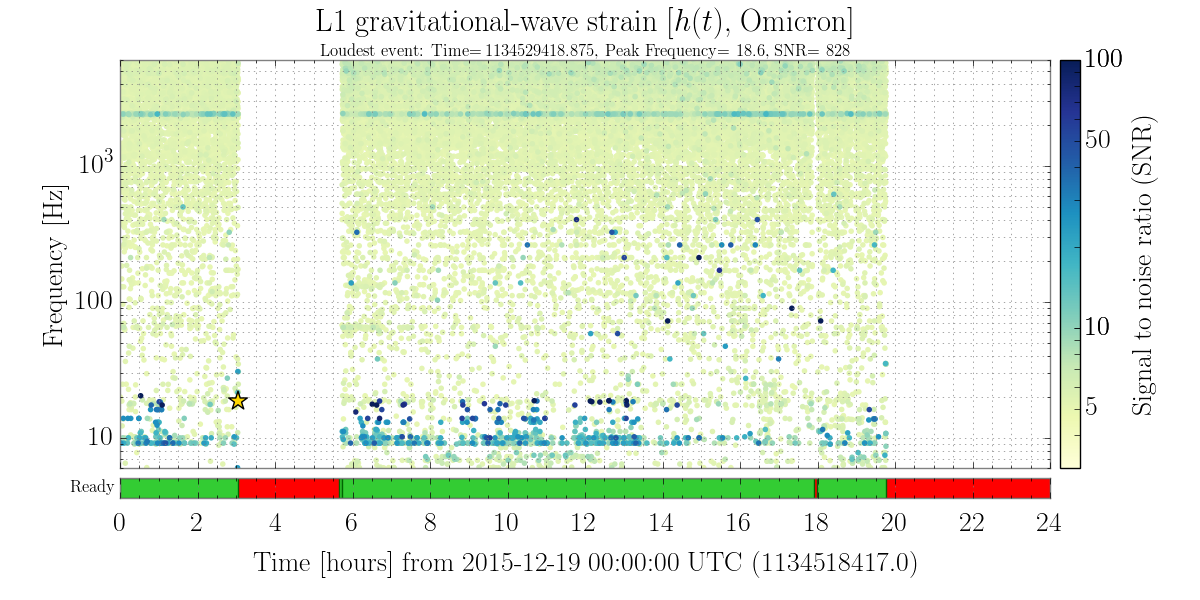
\includegraphics[width=\textwidth]{figures/detchar/Omicron-Dec19}
\caption[Omicron time-frequency-SNR plot]{Time-frequency-SNR plot of Omicron triggers.}
\label{fig:glitchgram}
\end{figure}

The results of Omicron are a commonly used and extremely valuable tool 
for characterizing the noise in the instrument. A cursory glance at 
Figure \ref{fig:glitchgram} identifies 3 populations of noise in 
the instrument, each of which can be followed up on individually 
to discover both the source of the noise and its effect on astrophysical 
searches. Omicron triggers can also be used in statistical analyses to 
find correlated noise between auxilary channels and $h(t)$. An often used 
example of this, Hierarchichal Veto, is discussed below. 

\subsection{Hierarchichal Veto}

One tool that we have often used in Detector Characterization to look 
for time coincidence between noise transients, or 'glitches', in auxilary 
channels and the output of the interferometer is Hierarchical Veto (Hveto). 
Typically, Hveto is used to compare a channel that potentially contains 
gravitational wave signals, denoted $h(t)$, and an auxiliary channel 
that does not have direct astrophysical implications. Hveto counts 
the number of coincident triggers between two time series using a 
user-defined time window centered around each trigger in the auxiliary 
channel. The figure of merit returned by Hveto for each auxiliary channel 
after comparison to $h(t)$ is called \textit{significance}.

Significance answers the following question: how unlikely is it that 
the coincident triggers in these two channels were the result of 
two arbitrary Poisson processes occurring in each channel? 
More specifically, given two arbitrary Poisson processes, how 
unlikely is it that we measure $n$ or more coincident triggers 
given that expected number of coincidences from random chance is $\mu$?

Significance is calculated as (ref Hveto),
\begin{equation}
S = -\log_{10} (\sum\limits_{k = n}^{\infty} P(\mu,k)),
\end{equation}
where $n$ is the number of coincidences found between the two channels 
during the total analysis time and $P(\mu,k)$ is the Poisson probability 
distribution function,
\begin{equation}
P(\mu,k) = \frac{\mu^{k}e^{-\mu}}{k!},
\end{equation}
where $\mu$ is the expected number of coincidences between triggers in 
$h(t)$ and the auxiliary channel based solely on chance, which is estimated as,
\begin{equation}
\mu = \frac{N_{h}N_{aux}T_{win}}{T_{tot}},
\end{equation}
where $N_{h}$ and $N_{aux}$ are the number of triggers in $h(t)$ and a 
given auxiliary channel respectively, 
$T_{tot}$ is the total analysis time, and $T_{win}$ is the length of the 
coincidence window used.

A high value of significance indicates that the triggers in the channels 
were very often coincident in time and that there is a very small probability 
that their intersection is a product of random chance. This is a very useful 
measure when we are searching for auxiliary channels that might have some 
noise coupling into our output channel. A significance value of up to 5 is 
often observed in channels with no causal relationship to $h(t)$ (ref Hveto), 
which is a useful threshold for identifying effective vetoes.

Another interesting figure of merit used for a given comparison Hveto is 
the ratio of $\frac{efficiency}{deadtime}$. Efficiency is defined as the 
percent of triggers vetoed from $h(t)$ during a round of vetoes. Deadtime 
is defined as the percent of total analysis time removed from $h(t)$ during 
a round of vetoes. A ratio of 1 is what we would expect from vetoing time 
at random, indicating no strong time correlation between triggers in the 
two channels. A high value of this ratio, which is ideal, indicates that 
we are vetoing a large number of triggers while maintaining a high percentage 
of our analysis time. This means that the triggers are often close enough 
in time that we can catch a large number of triggers using a small time window.

The deeper utility of Hveto is made evident when a channel is found to have 
a strong correlation with $h(t)$. 
When Hveto discovers an auxiliary channel that has a strong correlation 
with $h(t)$, which is called the round winner, it removes all of the time 
windows surrounding 
auxiliary channel glitches and recalculates the significance of the list of 
auxiliary channels. If a channel's significance has dropped after this removal 
of time, it must have had a large amount of glitches coincident with the 
round winner. The change in significance of each channel is displayed on a 
figure called a `drop-plot`. This is one of the most powerful features of Hveto
 - the ability to find families of channels that often glitch at the same time. 

Ideally, the list of significant channels displayed on the drop-plot will be 
able to localize the issue to a specific subsystem or area of the IFO. 
For example, if a channel representing the alignment of the input mode 
cleaner has glitches that are strongly correlated to $h(t)$, it would be 
interesting to look at the drop-plot and find out what other channels are 
glitching at the same time (suspensions, laser power, etc.).
From there, the issue can be investigated and brought to the attention of 
commissioners for repair or physical inspection. This is not always possible 
as sometimes the cause of the glitches is unclear, but identifying times of 
poor data quality is still useful.

Using Hveto, we can monitor auxiliary channels to find and remove glitches 
in $h(t)$ that would otherwise pollute a gravitational-wave analysis. Removing 
these glitches serves multiple purposes for the search pipelines. Removing 
high SNR glitches cleans up search backgrounds and allows the search 
pipelines to claim a lower SNR threshold for potential detections. A lower 
SNR threshold implies a larger volume for astrophysical analysis. Removing 
glitches reduces the potential for false alarms in the search pipelines, 
which in turn increases the confidence of eventual detections.

\section{Instrumental Detector Characterization Studies}

\subsection{Analog-to-Digital Conversion}

Advanced LIGO interferometers are controlled in real-time using a digital 
control system installed on a series of computers referred to as front end 
computers.  This system overall is referred to as the Front End Control 
(FEC) subsection of the more expansive Control and Data System (CDS).  
In a control loop, the FE computers must be capable of reading in an 
analog signal from the interferometer (position measurements, error signals, 
coil currents, etc), digitally sampling that analog signal, using these now 
digital values in a series of control algorithms, and outputting an analog 
control signal to send back into the interferometer.

The process of digital sampling is handled by an analog-to-digital 
converter (ADC) and the process of analog output is handled by a 
digital-to-analog converter (DAC).  Since these converters are linearly 
mapping a continuous signal onto a discrete range, they are limited by 
their digital bit depth.  For example, a 16 bit ADC is only capable of 
representing $2^{16}$ discrete values, or a range from zero to 65536.  
This range is often centered around zero, giving the ADC the capability 
to handle a range of $\pm32768$.  An incoming analog signal is mapped 
onto this range and converted into a digital signal.

For example, in sampling an analog signal with a range of $\pm20V$, 
10V would be mapped to 32768 digital counts and -10V would be mapped 
to -32768 digital counts with all 
of the intermediate voltage values being linearly mapped to the range. This 
means our digital system would recognize a discrete step size of 
10V/32768 counts $\approx 305 \mu $V/count.

Looking at the system described above, we must be aware of how our system 
is going to react when our analog input signal exceeds the intended maximum 
value of 10V (e.g., an 11V input). The ADC has already assigned its maximum 
digital value to 10V. This is called a digital overflow. In this case the ADC 
will continuously output its maximum value as it has no way to map 11V into 
a discrete value. The same process can occur in a DAC when a digital signal 
is sent out at the maximum allowed digital value. The resulting analog signal 
will be railed at the maximum output value of the DAC, creating a sharp corner 
in the output signal as it flattens out. 

If the digital system is not able to correctly sample and understand an analog 
error signal, it is easy to imagine a scenario where the reponse of the digital 
system and the output control signal are not able to complete the control loop 
as designed. This may cause glitches or misalignments in the interferometer.
We must also consider the fact that many ADCs are calibrated to reflect the 
intended dynamic range of an optic.  If a saturation is occurring, there is 
a good chance that an optic has moved beyond this intended dynamic range, which 
also may cause glitches or misalignments.

The ADCs and DACs are monitored by a series of auxiliary channels, which are 
automatically generated in the front-end system. These auxiliary channels 
monitor each ADC and DAC channel and note when any of the channels has reached 
its digital limit. These channels can be used to generate flags that mark 
ADC and DAC overflows, which can be compared with glitches in $h(t)$ to 
search for glitch mechanisms driven by overflows. These channels can also 
be used to flag any large glitches that cause digital overflows so that they 
can be removed from astrophysical searches. 

Figure \ref{fig:dac-overflow} shows an example of a large glitch that caused 
a digital overflow and was removed from gravitational wave analyses. Figures 
\ref{subfig:strain-dac-overflow} and \ref{subfig:esd-dac-overflow} show a 
large glitch in $h(t)$ and the response of a drive signal that controls 
the motion of ETMY respectively. The signal in \ref{subfig:esd-dac-overflow}, 
which is supposed to be controlling the motion of ETMY, hits its digital 
limit during this glitch. Figure \ref{subfig:etmy-dac-overflow} shows the 
auxiliary channel that monitors this digital overflow incrementing as 
it witnesses the digital overflow. 

\begin{figure}[ht!]%
\centering
\subfloat[]{
  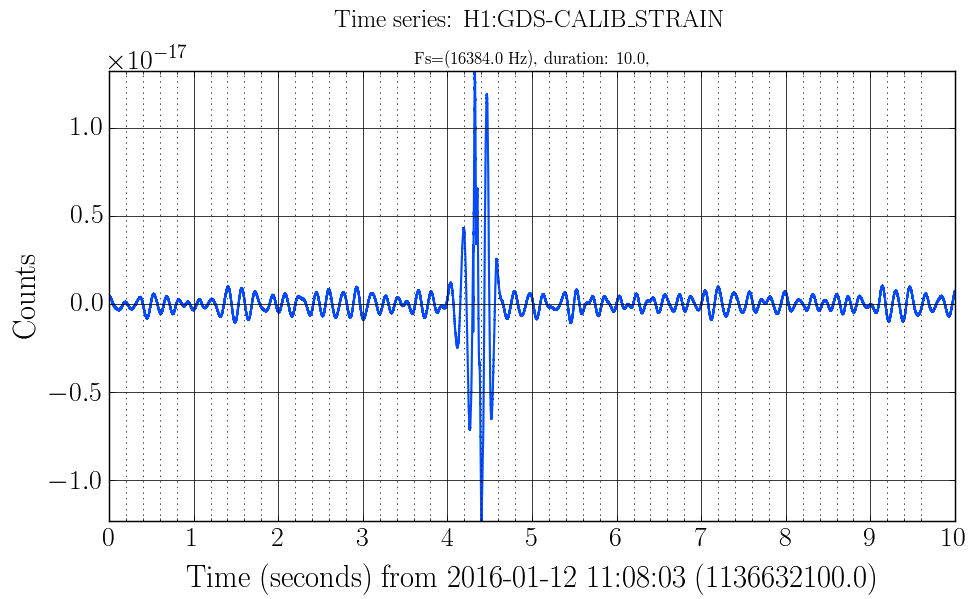
\includegraphics[width=0.495\textwidth]{figures/detchar/strain-dac-overflow}
  \label{subfig:strain-dac-overflow}
  }
\subfloat[]{
  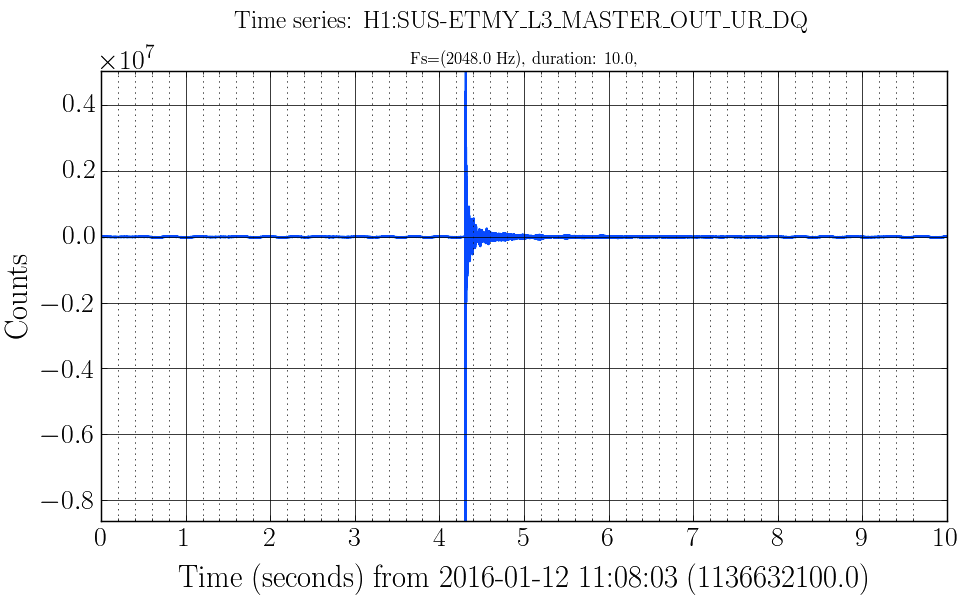
\includegraphics[width=0.495\textwidth]{figures/detchar/esd-dac-overflow}
  \label{subfig:esd-dac-overflow}
  }

\subfloat[]{
  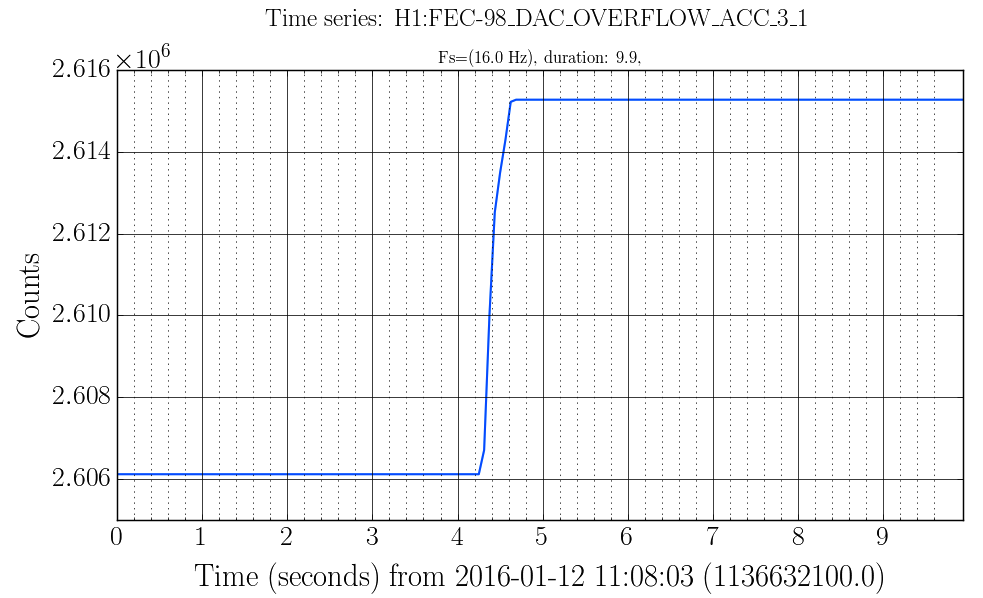
\includegraphics[width=0.495\textwidth]{figures/detchar/etmy-dac-overflow}
  \label{subfig:etmy-dac-overflow}
  }
\caption[ETMY saturation]{Timeseries of an ETMY drive signal saturation in the 
         H1 detector. Figure \ref{subfig:strain-dac-overflow} shows a glitch in 
         the calibrated $h(t)$ channel. Figure \ref{subfig:esd-dac-overflow} shows 
         the response to this glitch in the drive signal used to control the bottom 
         stage of ETMY and actuate on the DARM degree of freedom. This signal hits 
         its digital overflow point at its peak and has no more dynamic range. 
         Figure \ref{subfig:etmy-dac-overflow} shows the front end channel responsible 
         for monitoring digital overflows of this particular ETMY drive signal. 
         Since the witness channel is cumulative, overflows can be identified by 
         flagging any time in which this witness channel is increasing. }
\label{fig:dac-overflow}
\end{figure}

This method was used throughout O1 to generate data quality vetoes that 
were distributed to the Burst and CBC searches. The first veto that was 
generated this way was used to flag DAC overflows of the ETMY drive signal, 
as demonstrated 
in Figure \ref{fig:dac-overflow}. The other veto generated in this framework 
was used to flag ADC overflows in the OMC DC photodiode used as the error 
point of the DARM control loop. 

\subsection{Suspension DAC calibration glitches}

A common glitch mechanism throughout ER6 was due to calibration errors in 
digital-to-analog converters (DACs) responsible for providing analog signals 
to the aLIGO suspensions. The aLIGO suspension subsystem uses 18-bit DACs 
to interact with the optics in the interferometer. These 18-bit DACs are 
created by combining a 16-bit DAC with a 2-bit DAC inside of the same 
electronics box. The 2-bit DAC is responsible for the two highest order 
bits of the output, while the 16-bit DAC is responsible for the 16 lowest 
order bits of the output. If the 16-bit DAC and 2-bit DAC have not had 
their output voltages carefully calibrated, there will be a voltage discontinuity 
at the output of the DAC when engaging the 2 highest order bits. 

Since these DACs use the two's complement 
representation for signed binary numbers, there are two critical points 
where the two highest order bits of the DAC become necessary. The highest 
order bit is used to indicate negative numbers, so an output discontinuity 
is expected when transitioning from a positive number to a negative number, 
that is, crossing through a value of zero.  
The other bit from the 2-bit DAC is used to represent large output values and 
engages when the DAC needs to express a value which is unable to be 
represented by a 16-bit DAC alone. As such, we also 
expect to see discontinuities when the DAC output crosses $\pm2^{16}$. 

The fact that this discontinuity existed in suspension subsystem was 
particularly problematic, as the suspension DACs are used to directly 
actuate on mirror positions and optical cavity lengths. Any time a 
suspension DAC crossed one of these problematic output values, it would 
actuate on the optics with a step function and cause a glitch in the 
optical cavity length. Figure \ref{fig:DAC-glitch} shows an example of 
this issue where the DAC providing actuation signals to the power recycling 
mirror (PRM) is crossing through zero and there are associated glitches 
visible in the length readout of the power recycling cavity.

\begin{figure}[ht!]%
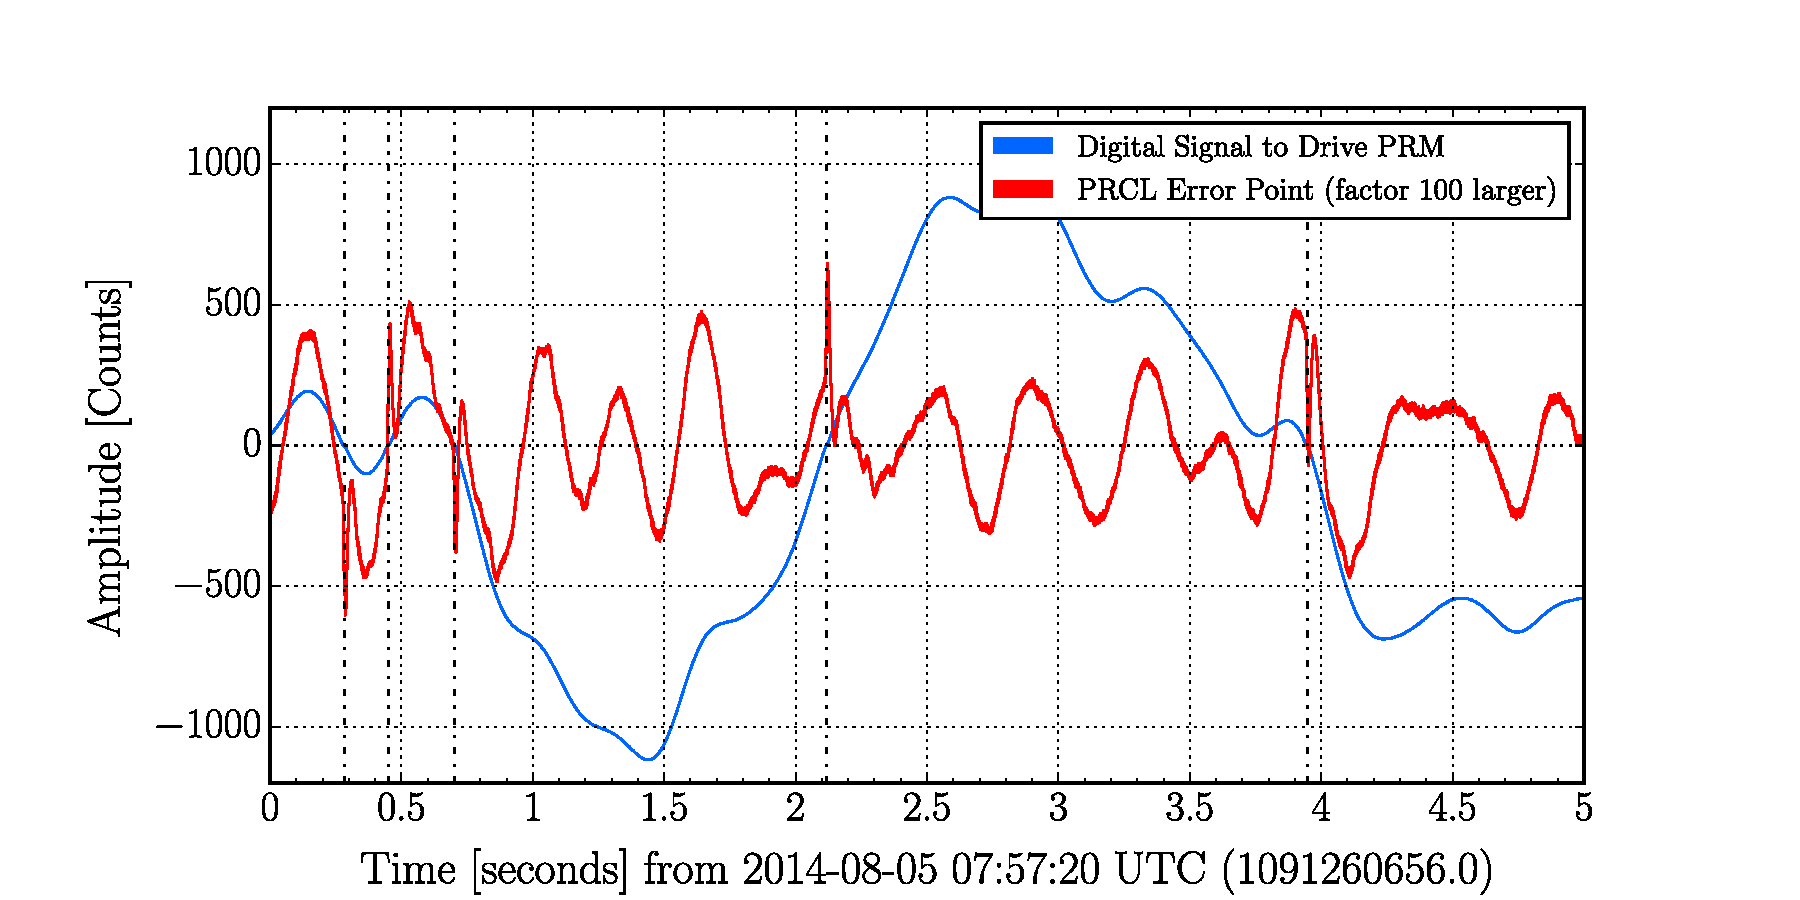
\includegraphics[width=\textwidth]{figures/detchar/PRCL-DAC-glitch}
\caption[DAC glitches in PRCL]{A timeseries plot showing the effects of %
         DAC calibration glitches. The red trace shows the digital drive %
         signal being sent to the digital-to-analog converter. The blue %
         shows the resulting power recycling cavity motion rescaled by a %
         factor of 100. When the drive signal crosses %
         through a value of zero, the output of the DAC experiences a %
         discontinuity, leading to a glitch in the power recycling cavity %
         length.}
\label{fig:DAC-glitch}
\end{figure}

The effects of this issue were visible in the $h(t)$ channel during ER6. 
The most problematic culprit was the DAC that applied actuation directly 
to the optics of the ETMs, effectively pushing directly on the DARM degree 
of freedom and causing glitches in $h(t)$. These calibration errors manifested 
themselves as a population of glitches in $h(t)$ recovered by Omicron in the 
20-100 Hz range. This is a very damaging frequency range for CBC searches, 
which hope to accumulate significant SNR in the region from 30-500 Hz.  
This population of low frequency glitches was obvious in an Omicron 
time-frequency scatter plot and was considered a significant noise source 
throughout the sixth engineering run.

Figure \ref{fig:vetoed-DAC} shows the result of an Hveto run that looked 
for time correlations between Omicron triggers in $h(t)$ and times when 
the ETMY drive signal crossed through a value of $2^{16}$. The blue dots 
represent all Omicron triggers in $h(t)$. The red crosses indicate those 
that were coincident with the ETMY drive signal crossing $2^16$. The 
population of low frequency glitches with SNR $>$ 8 was shown to be 
coincident with the drive signal transitions. This veto 
was very statistically significant, as shown in Table \ref{table:etmy-dac-hveto}. 
The significance 
of 192.5 indicates that the probability of these coincidences being due 
to noise alone is negligible. The effiency:deadtime ratio of 27 indicates 
that these glitches were removed with very small time windows (0.2s) 
and very little instrument uptime was removed in the process.

\begin{figure}[ht!]%
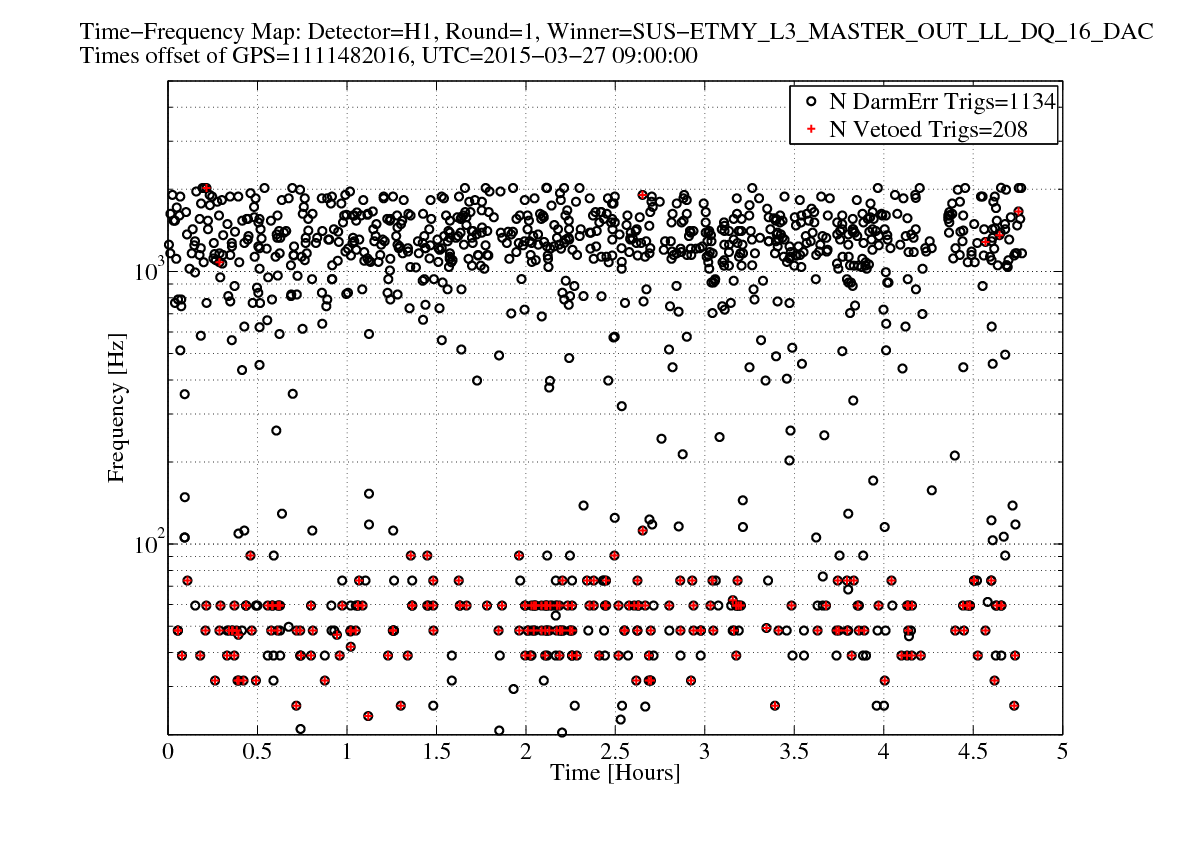
\includegraphics[width=\textwidth]{figures/detchar/vetoed-DAC-glitches}
\caption[Vetoed DARM triggers from DAC calibration]{A time-frequency %
         visualization of Omicron triggers in the H1 $h(t)$ channel. % 
         The black circles indicate glitches in the DARM degree of freedom, %
         each with a central time and central frequency. The red crosses %
         indicate that a given trigger was vetoed by an auxiliary channel %
         trigger which was found to be statistically significant using Hveto. The %
         auxiliary channel triggers in this case indicate that the drive signal %
         on the bottom stage of ETMY has crossed a value of $2^{16}$. The %
         population of glitches between 20 - 100 Hz is highly coincident %
         with these crossings of $2^{16}$, indicating that they are caused %
         by DAC calibration errors on this optic.}
\label{fig:vetoed-DAC}
\end{figure}

\begin{table}[ht!]%
 \footnotesize 
 \begin{center}
  \begin{tabular}{cccccc}
  \hline
  Channel & \begin{tabular}{@{}c@{}} Time \\ window (s) \end{tabular} & 
            \begin{tabular}{@{}c@{}}SNR \\threshold \end{tabular} & 
            Significance & Efficiency \% & Deadtime \% \\ 
  \hline
  \begin{tabular}{@{}c@{}}ETMY drive signal \\ crosses $2^{16}$ \end{tabular} & 
  0.2 & 8 & 192.5 & 18.3 &  0.674 \\
  \hline
  \end{tabular}
  \end{center}
  \caption[HVeto results for ETMY DAC glitches]{Hveto results for ETMY DAC glitches}
  \label{table:etmy-dac-hveto}
\end{table}

To fully understand the scope of this problem, the Detector Characterization 
group developed software that searched through the output of all suspension 
DAC digital output signals and marked times when they crossed 0 or $\pm2^{16}$. 
These marked times were converted into trigger files and sent through Hveto 
to look for correlations between crossings of critical values and glitches 
in DARM as identified by Omicron. Through this method, we were able to identify 
which optics were experiencing DAC calibration glitches that had a coupling 
mechanism into DARM.

There were two approaches taken in an effort to mitigate these DAC glitches. The 
first was to introduce offsets into the suspension drive signals so that they 
did not cross through a value of zero. This did solve the problem temporarily, 
but at the cost of a significant portion of the dynamic range of the output 
actuation. The more permanent fix was to run a calibration routine 
that resolved the issue between the 16-bit and 2-bit DACs. This was 
successful, though it had to be run on a weekly basis during site maintenance 
because the calibration tended to drift away from its nominal point after 
2-3 weeks of operation.

During the first observing run, the systematic check of all suspension DAC 
digital output signals was performed again and the resulting triggers were 
sent through Hveto. This study revealed that the calibration process was 
successful; there was no evidence of residual DAC calibration glitches that 
had any noticeable coupling into $h(t)$. The only signal that had any 
significant correlation with glitches in $h(t)$ was not causally sensible. 
Large glitches $h(t)$ were driving the ETMX actuation signal through a value of 
$2^{16}$, which resulted in crossings of $2^{16}$ that were coincident in time 
with glitches in $h(t)$, but weren't representative of calibration errors.

\textcolor{red}{Discuss Hveto results}

\subsection{RF beatnote whistles}

Two RF oscillators beating against one another creates a kHz beatnote that couples 
into DARM.

\begin{figure}[ht!]%
\centering
\subfloat[]{
  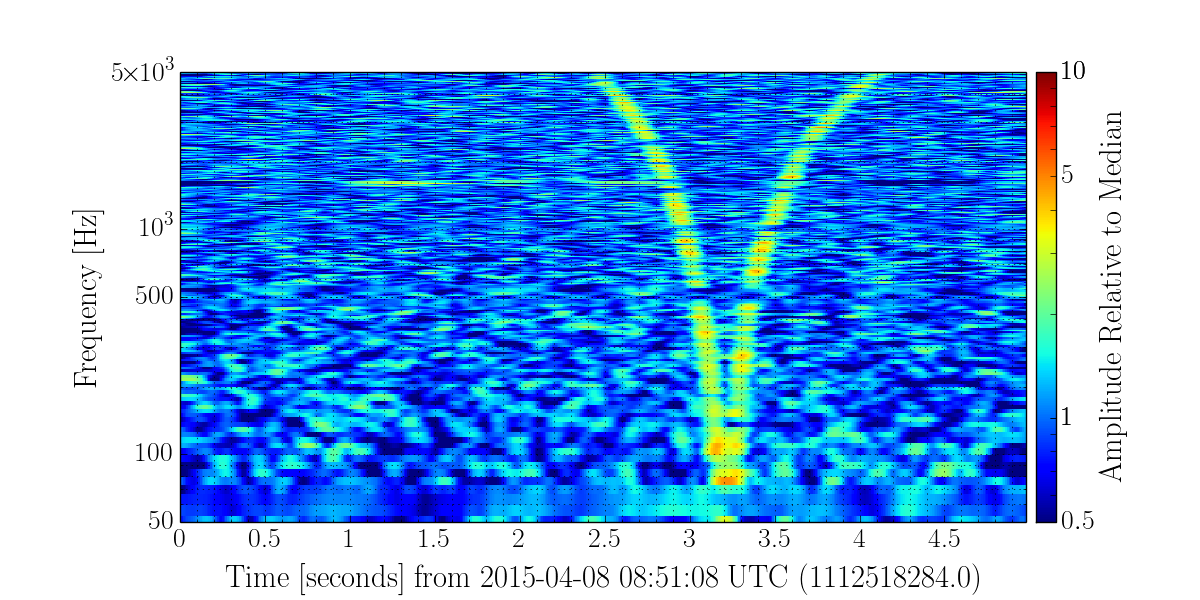
\includegraphics[width=\textwidth]{figures/detchar/Spectrogram_Whistle_LLO}
  \label{subfig:llo-whistle}
  }
  
\subfloat[]{
  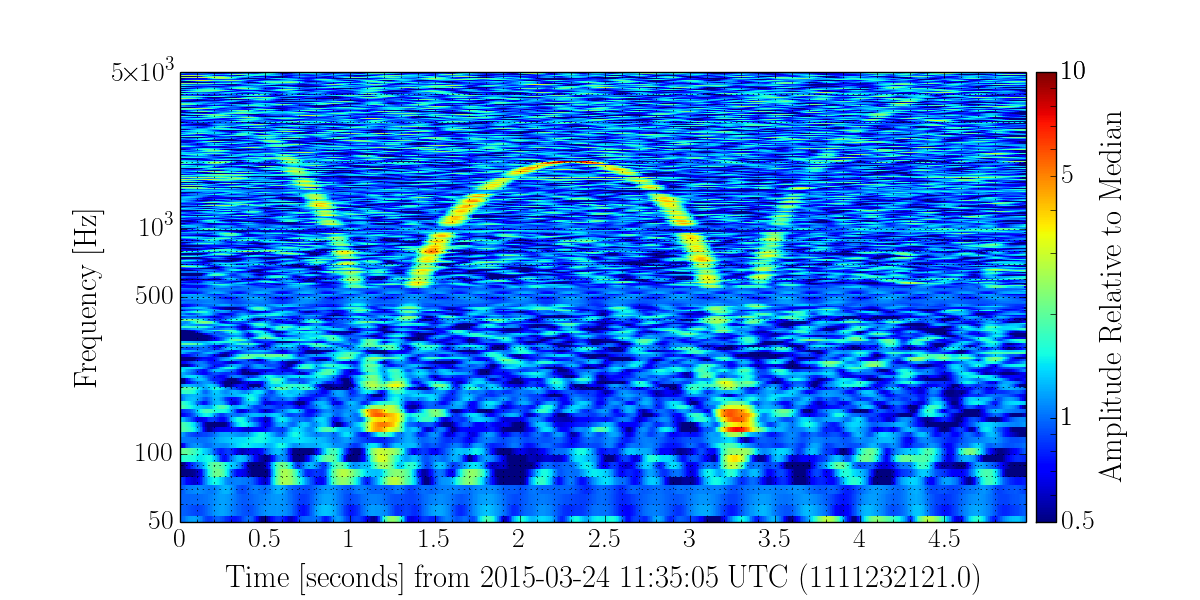
\includegraphics[width=\textwidth]{figures/detchar/Spectrogram_Whistle_LHO}
  \label{subfig:lho-whistle}
  }
\caption[Spectrograms of RF whistles]{Time-frequency spectrograms of RF whistles at %
         both LLO and LHO. Figure \ref{subfig:llo-whistle} shows a %
         whistle at LLO sweeping down from the kHz range and into the detection band %
         where it interferes with searches for gravitational waves. Figure %
         \ref{subfig:lho-whistle} shows a double whistle whistle at LHO where the %
         two oscillators drifted back and forth across one another and caused two %
         glitches in the detection band.}
\end{figure}\label{fig:whistle-spectrograms}

Hveto shows that a witness channel for RF whistles vetoes approximately 90\% 
of DARM triggers in this time period.

\begin{figure}[ht!]%
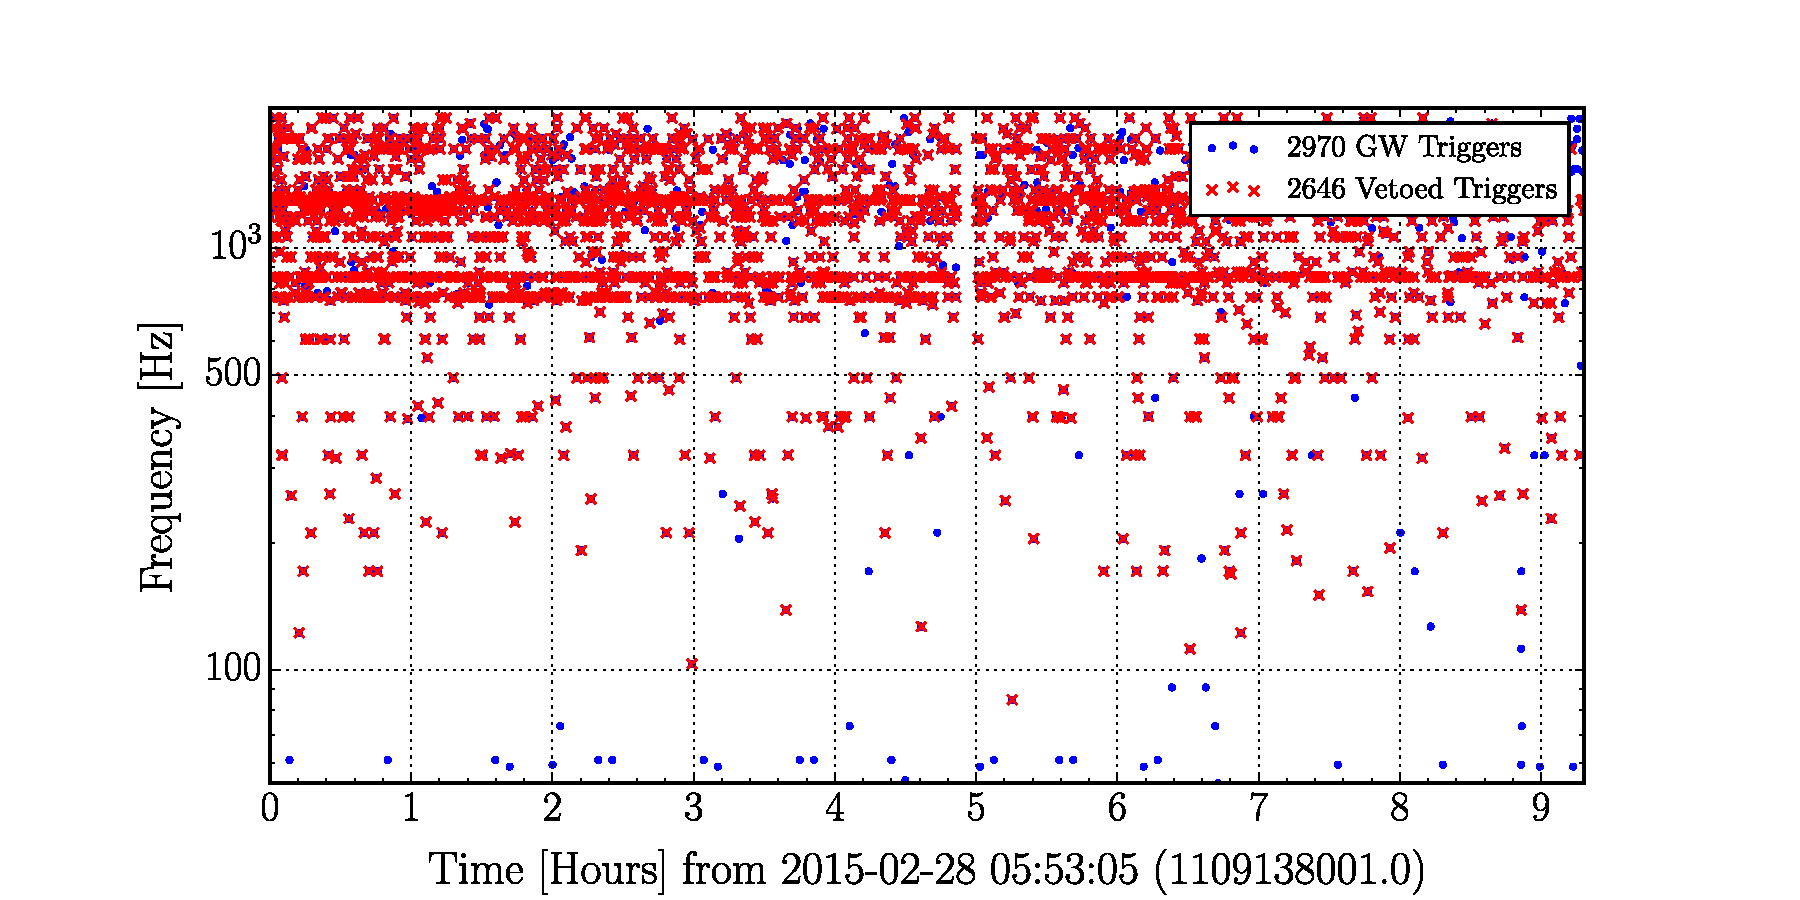
\includegraphics[width=\textwidth]{figures/detchar/Hveto_whistles_time_frequency}
\caption[Vetoed whistles from Hveto]{A time-frequency scatter plot of $h(t)$ Omicron %
         triggers. The blue dots represent all triggers found for the $h(t)$ channel. %
         Red crosses indicate that a trigger was determined to be coincident with an %
         RF whistle and vetoed. This veto is responsible for removing 90\% of the %
         glitches in this time period. The majority of the high frequency glitches %
         were due to RF beatnote whistles}
\end{figure}\label{fig:hveto-whistles}

How do we know that the frequency offset worked? Look at a signal that is a proxy 
for the drifting oscillator and histogram all of the Omicron DARM triggers during 
that time. If there's no coupling, the answer should be fairly Gaussian; the 
IFO is just as likely to glitch at any value of the channel. If there are 
channel values that correspond strongly to glitches in DARM, we should see peaks.

\begin{figure}[ht!]%
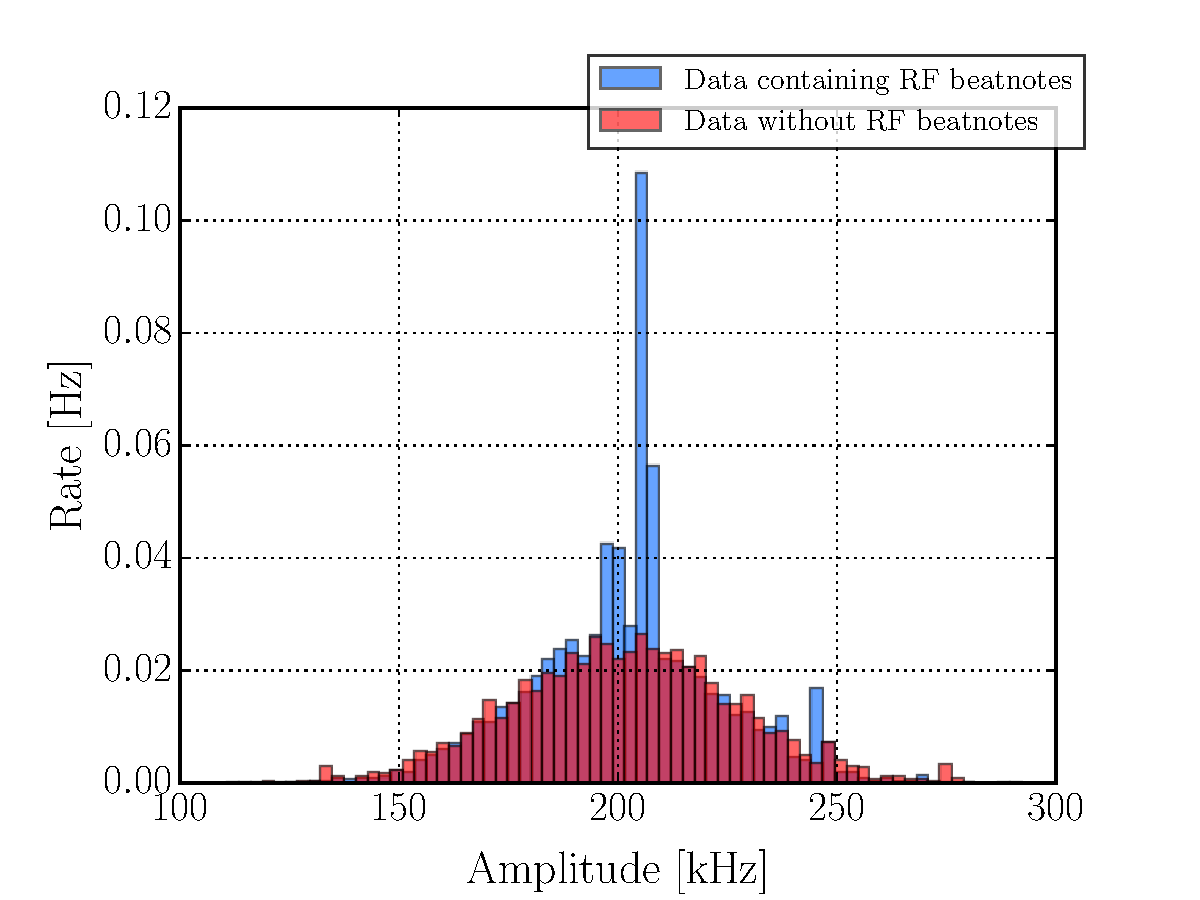
\includegraphics[width=\textwidth]{figures/detchar/Rate_Histogram_Whistles_LLO}
\caption[DARM glitch histograms with and without RF whistles]{Red curve is nice %
         and Gaussian. Blue curve has peaks that indicate problematic frequencies.}
\end{figure}\label{fig:darm-whistle-hist}

\subsection{Seismic CPS comb}

Oscillators in the capacitive position sensors had drifted apart and caused a 
beatnote and a comb. Audio analysis pointed towards amplitude modulation. 

Fixed by slaving all oscillators to a master.

\subsection{DC values of auxiliary channels}

No great correlation at the end of the day 

\subsection{Earthquakes during full lock}

Lots of scattering arches during an earthquake, drove up the noise and biased PSD.
Caused a sarlacc, removing this data was able to repair data on either side.

\subsection{L1 PMC glitches}


Characterization of noise and analysis after repair

\subsection{Data quality shifts}
Performed and mentored data quality shifts.




\Chapter{IMC Upconversion}
\label{ch:IMCUpconversion}
\section{Abstract}

LIGO interferometers use several high finesse optical cavities for gravitational wave detection. The lengths of these cavities are controlled using radio frequency (RF) modulation-demodulation techniques in a Pound-Drever-Hall (PDH) locking scheme. This scheme provides a PDH error signal that is linear to cavity length over a specific range. This study examines the specific case of the triangular ring cavity uses in LIGO interferometers for input mode cleaning. When the length of the cavity approaches the boundaries of the PDH error signal linear range, our model of the input mode cleaner PDH response shows that the resulting error signal contains non-linear spectral artifacts. This model and understanding of the non-linear cavity responses will be useful in the commissioning phase of the Advanced LIGO project for more precisely locating and eliminating systematic noise sources in the interfereometers

\section{Model}

The PDH response of the cavity was modeled using measured values of optical reflectivity and free spectral range of the Livingston input mode cleaner. The input beam was the nominal LIGO carrier beam with a frequency of $\omega = 281.8$ THz ($\lambda = 1064$ nm) and modulation sidebands of $\Omega = \pm24$ MHz.

The reflection coefficient of a LIGO input mode cleaner as a function of input beam frequency is given as,

\begin{equation}
F(\omega) = \frac{r(1 + e^{-i\phi})}{1+r^2e^{-i\phi}} = \frac{r(1 + e^{-i(\frac{\omega}{\nu_{fsr}})})}{1+r^2e^{-i(\frac{\omega}{\nu_{fsr}})}}
\end{equation}

where $r$ is the reflectivity of the input mirror, $\phi$ is the round-trip phase accumulated when traversing the cavity, and $\nu_{fsr}$ is the free spectral range of the cavity \cite{Mueller}.

In a situation where the carrier beam is resonant in the cavity and the modulation sidebands are high enough in frequency that they are not resonant, the PDH error signal, here denoted $\epsilon$ is given as

\begin{equation}
\epsilon(\omega) = -2\sqrt{P_{c}P_{s}}\operatorname{Im}\{F(\omega)F^*(\omega + \Omega) - F^*(\omega)F(\omega - \Omega)\},
\end{equation}

where $P_{c}$ is the the carrier beam power and $P_{s}$ is the sideband power \cite{Black01}.

Note: the above error signal is a function of laser frequency. This is an artifact of the original intent of PDH locking: using a fixed length resonant cavity to control the frequency of a laser by forcing it to match the cavity length. We can apply the same technique but flip the direction of feedback and use a highly stable laser to control the length of a free swinging resonant cavity by pushing on the mirrors to match the cavity length to the laser wavelength. The laser frequency detuning and cavity length detuning are linearly mapped to one another using the free spectral range of the resonant cavity.

Importantly, this error signal is linear to the length of the IMC within a certain range of motion. If the optics begin swinging too far away from the nominal locking point, we will begin to see a non-linear response and eventually a lock loss.

To explore this non-linearity, we injected a sinusoidal cavity motion into our model and observed the resulting error signal.

We explored two specific cases. Figure 1 shows spectra of the injected sinusoidal cavity motion (green) and the resulting non-linear error signal (blue). This motion was injected asymetrically about the nominal cavity locking point ($\epsilon = 0$) and therefore we see both even and odd harmonics of the injection frequency.

Figure 2 shows spectra of the injected sinusoidal cavity motion (green) and the resulting non-linear error signal (blue). However, this time the motion was injected symetrically about the nominal cavity locking point and as a result we only see odd harmonics of the fundamental frequency.

We hope to use this model as an explanation of systematic noise found in the aLIGO IMC.

\begin{figure}[h!]
\caption{Sinusoidal cavity motion with frequency 2.78 Hz injected asymmetrically about the locking point of the cavity results in a PDH error signal containing non-linear spectral artifacts at harmonics of the injected cavity motion.}
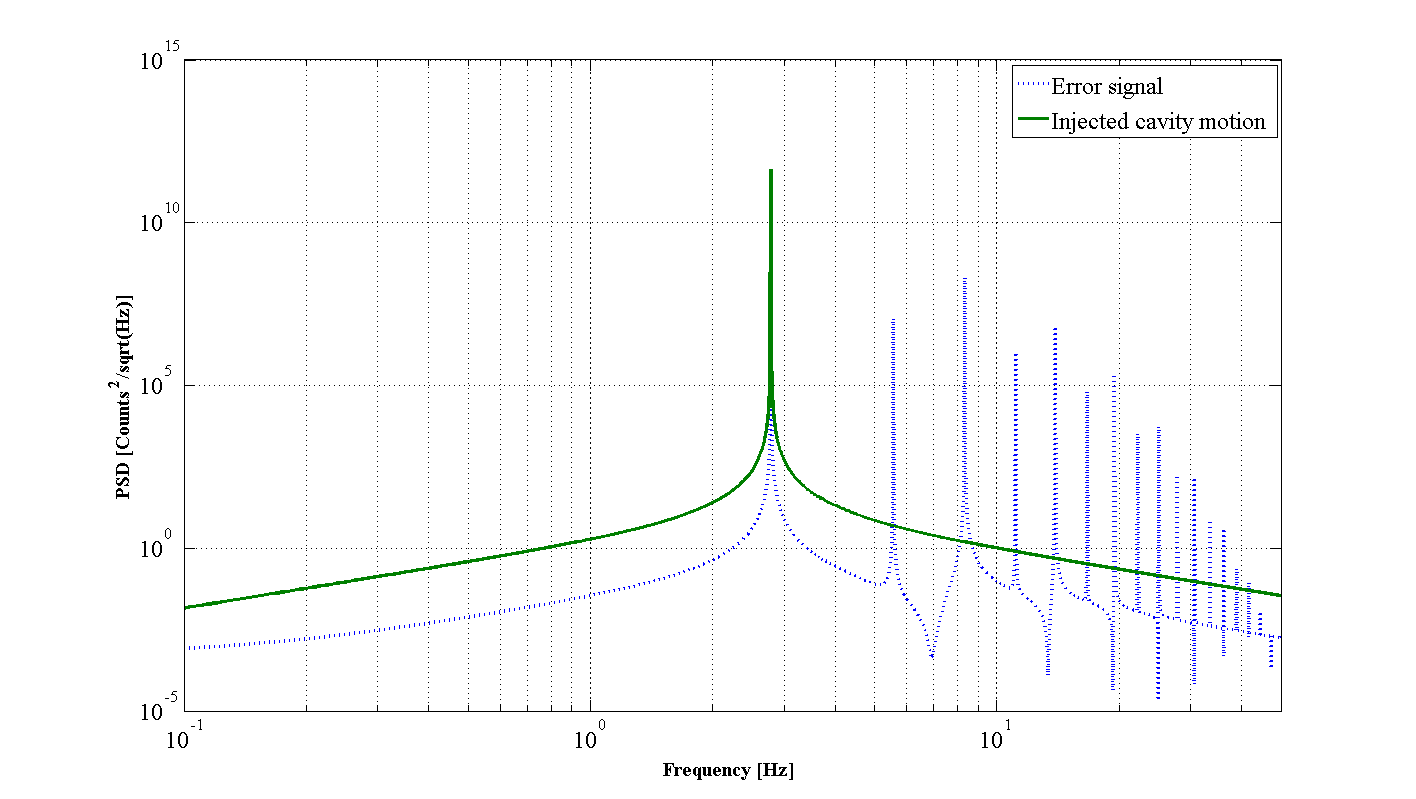
\includegraphics[height=0.6\textwidth]{figures/IMCUpconversion/PDH_error_signal_harmonics.png}
\end{figure}

\begin{figure}[h!]
\caption{If the motion is symmetric about the cavity locking point, we see only odd harmonics of the injection frequency.}
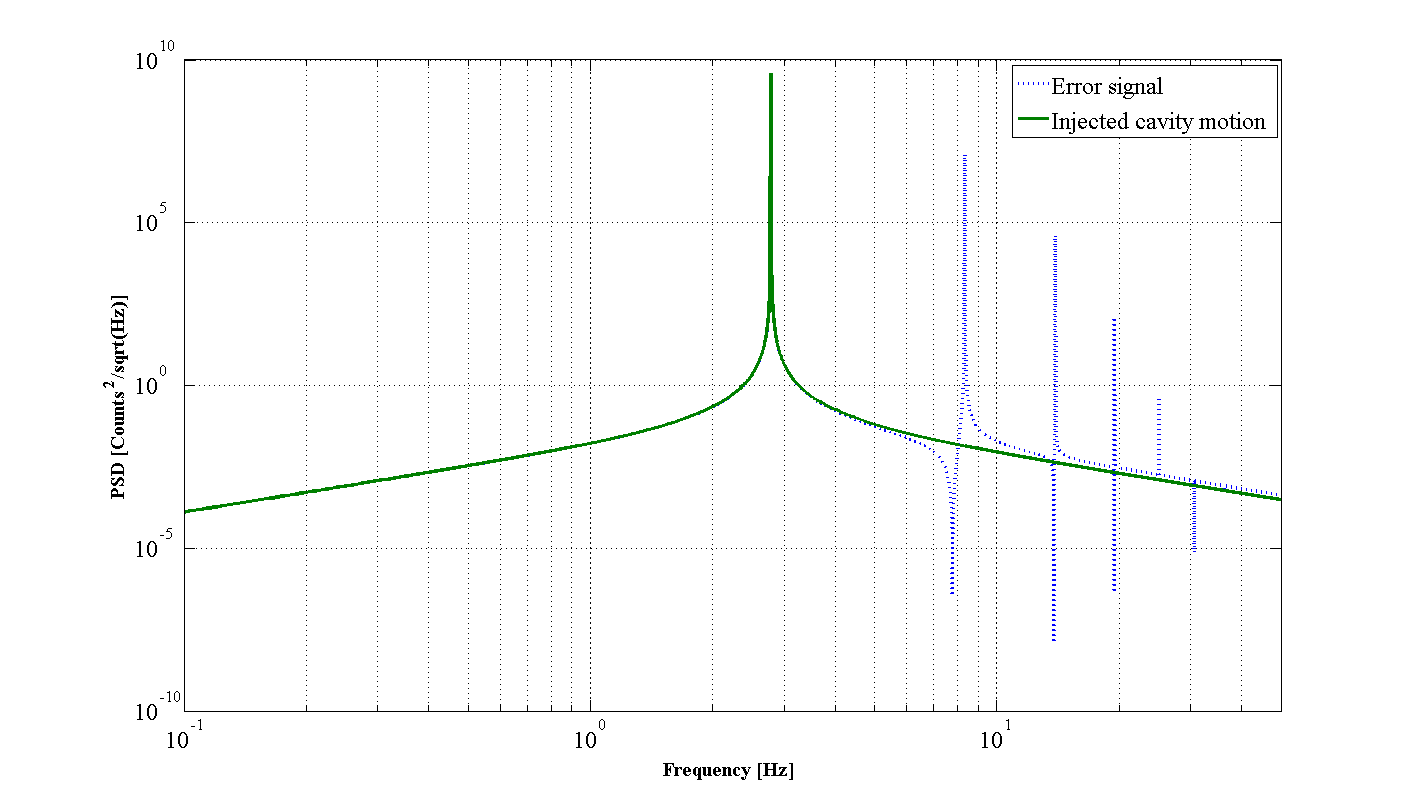
\includegraphics[height=0.6\textwidth]{figures/IMCUpconversion/symmetric_PDH.png}
\end{figure}

\section{Upconversion noise in aLIGO}
The aLIGO input mode cleaner (IMC) is a triangular ring cavity whose length is sensed and controlled using the PDH locking technique. Each of the three mirrors in the cavity is staged as the bottom mass of a triple suspension in order to passively isolate the mirrors from  potential noise sources. In addition, the chambers holding the IMC mirrors are isolated from ground motion by two stages of active seismic isolation. This isolation, however, is not completely impervious to external excitations. During periods of time with excess ground motion we can see seismic noise coupling into the cavity length and its control signal.

Specifically, when we see excess seismic noise in the 1-5 Hz anthropogenic band (believed to be caused by a commercial railroad a few kilometers from the LIGO Livingston Laboratory), we see highly structured noise in the IMC control signal in the 10-100 Hz band. This physical mechanism is consistent with the idea of a PDH range saturation. If excess seismic motion reaches the suspension and the optics begin swinging around, it's feasible that they could start to saturate the linear range of the PDH loop.

The noise takes a form very similar in structure to the non-linear PDH signal, displaying strong odd harmonics and weaker even harmonics. The IMC control signal has an associated noise floor that obscures parts of these peaks. The theoretical model uses sinusoids with a highly specified frequency and thus displays very sharp peaks in its spectrum. It should be noted that the peaks in the IMC control signal are the manifestation of a physical process, not digitally generated, and have some natural width to them.

\begin{figure}[h!]
\caption{Spectral comb with a fundamental frequncy of 2.78 Hz in the IMC control signal. Red arrows indicate odd harmonics, green arrows indicate even harmonics. }
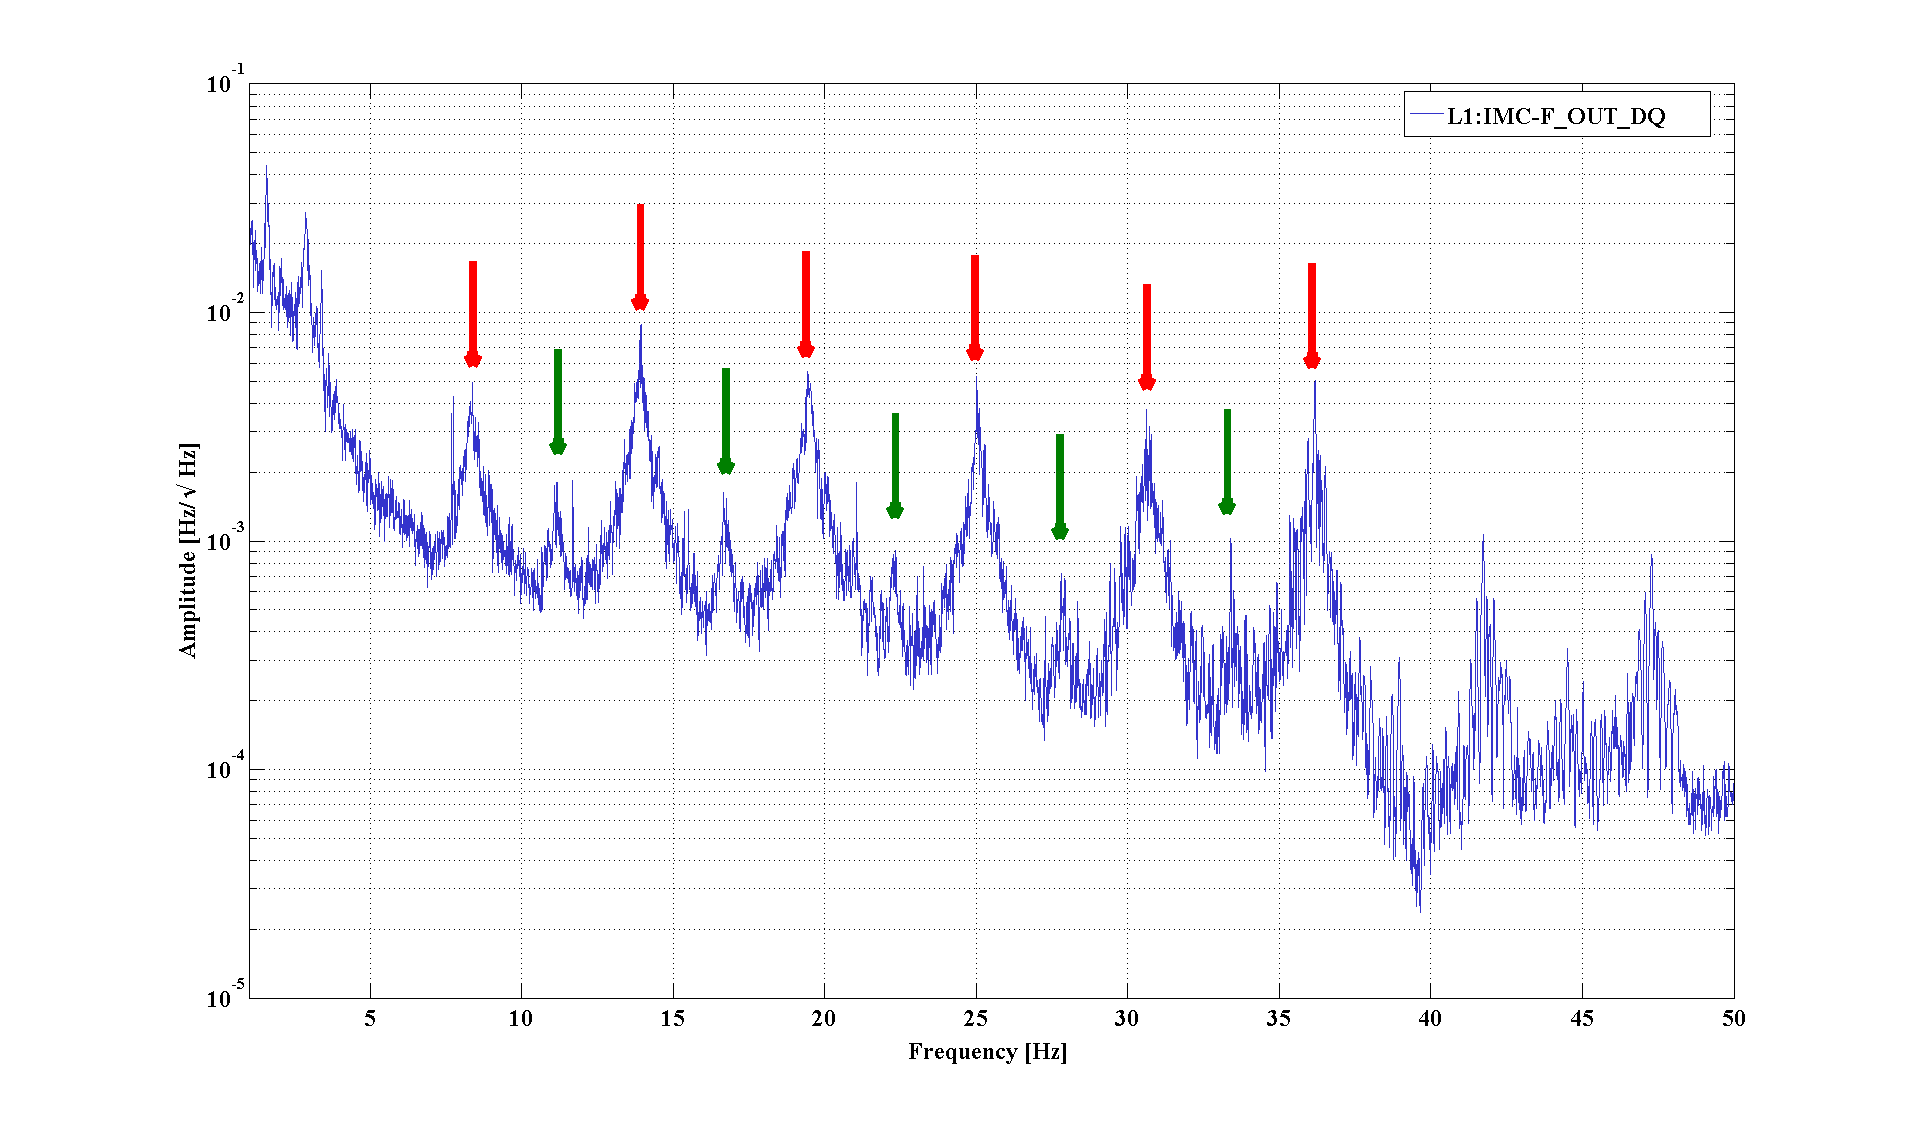
\includegraphics[height=0.6\textwidth]{figures/IMCUpconversion/upconversion_comb.png}
\end{figure}

\section{Next steps}

While we have demonstrated that this mechanism is a feasible explanation for the IMC upconversion noise, it has not yet been fully proven. We are currently looking for a better way to look at the actual IMC error point during times of excess seismic motion instead of the control signal. 

We also need to localize the source of the 2.78 Hz excitation. Why that specific frequency when the excess seismic noise is spread across a 1 - 5 Hz band? We think the source may be a vertical resonance of the triple pendulum suspension that houses the IMC optics being rung up by the excess motion.

We are also going to use the increasing full IFO uptime to figure out whether or not this upconversion noise is coupling downstream into critical cavities such as the recycling or arm cavities.

\section{Conclusions}

We found that injecting sinusoidal cavity motion into our input mode cleaner PDH model generates an error signal with non-linear spectral artifacts, specifically harmonics of the injection frequency, if the cavity motion exceeds the linear PDH range. For cavity motion that is symmetric about the locking point of the error signal, we find that the error signal contains only odd harmonics. For asymmetric cavity motion we find both even and odd harmonics, where the odd harmonics are typically higher in amplitude. In such a case, the amplitude of the even harmonics increases as the DC offset from the nominal locking point increases, that is, as the cavity motion is more asymmetric.


\Chapter{Online Detector Characterization}
\label{ch:ODC}
The aLIGO interferometers are highly complex, high precision devices. 
Their operation depends on the careful interaction of a series of subsystems, 
each with its own purpose. In an effort to better understand the operation 
and output of the interferometers, the Detector Characterization group has 
been designed to mirror this subsystem approach. Table 
\ref{table:aligo-subsystems} lists the aLIGO subsystems. Each of these 
subsystems is assigned a data quality liaison from the DetChar group. 

\begin{table}[ht!]%
  \begin{center}
    \begin{tabular}{|c|l|}
    \hline
    Subsystem & Description \\
    \hline
    LSC & Length Sensing and Control \\
    \hline
    ASC & Alignment Sensing and Control \\
    \hline 
    SUS & Suspensions \\
    \hline
    IMC & Input Mode Cleaner \\
    \hline 
    OMC & Output Mode Cleaner \\
    \hline
    PCAL & Photometric Calibration \\
    \hline 
    PEM & Physical Environmental Monitoring \\
    \hline
    SEI & Seismic Isolation \\
    \hline
    PSL & Pre-Stabilized Laser \\
    \hline
    TCS & Thermal Compensation System \\
    \hline
    \end{tabular}
  \end{center}
  \caption[Table of aLIGO subsytems]{Table describing aLIGO subsystems}
  \label{table:aligo-subsystems}
\end{table}

There are 5 main responsibilities assigned to a subsystem liaison. The 
first is to fully understand the operation and installation of the subsystem 
so that they can faciliate data quality investigations and act as a 
point of contact for commissioners assigned to this subsystem.

The second responsibility 
is to take this knowledge and use it to populate the channel information 
system (CIS), which is a database that stores information about how to 
parse and understand the various auxiliary channels that are monitored 
in each subsystem. This database also contains information about calibration 
and valid frequency ranges for these channels. This allows newcomers to the 
collaboration to more easily familiarize themselves with the LIGO naming 
conventions and facilitates their involvement in data quality investigations.  

The third responsibility 
is to check for signal fidelity, which means to make sure that all of the 
channels are working as intended and don't contain artifacts from signal 
conditioning processes.

The fourth responsibility is to develop summary pages that monitor 
important channels and figures of merit for each subsystem. 
The summary pages are generated 
every day from a configuration file designed by the subsystem liaisons. 
The purpose of the summary pages is to gather all of the potentially 
useful information about a subsystem in an organized way so that the 
subsystem leads can efficiently evaluate the performance of the subsystem. 
They are also a useful launch point for data quality shifts and 
investigations since they provide various overviews of instrumental 
performance ($h(t)$ spectrograms, Omicron triggers, BNS inspiral range, etc.) 
that make it easy to identify persistent or egregious data quality issues.

The fifth and final responsibility is to develop and build real-time 
data quality monitors in the Online Detector Characterization (ODC) 
framework. 
The Online Detector Characterization (ODC) system is an infrastructure designed
to extract and record metadata describing the state of the aLIGO interferometers.
This state information has two main purposes: to inform data quality investigations
by the DetChar group and to serve as a real-time monitor of the interferometer state
that can be accessed in the control room. Each subsystem monitored by the DetChar group
using an ODC monitor.

The ODC system is unique in that it is runs in real-time in the front-end control
system that is used to control the aLIGO interferometers. Each set of ODC monitors
is built in Simulink to directly interface with the models that run on the front-end
computers. This has several distinct advantages.
Since the monitors are run in real-time, they operate in parallel with the control
loops that are sensing the various degrees of freedom of the interferometer and are
able to achieve highly precise timing. The ODC monitors can also create their own
test points, which means an ODC monitor can perform a check on any signal that exists
in the front end at its full rate instead of relying on the information that is
downsampled and stored in frames.
These full rate test points operate at the full sample rate of the model (16384 Hz)
and any information recorded in the ODC channel is written at the same rate. In contrast,
many channels are only recorded at 16 Hz if they aren't accessed as a test point in the front-end system.

The information generated by each ODC monitor can be extracted and sent to a segment
generation process, where the most useful information is catalogued and represented by
segments of time that indicate when a given flag was considered to be active.

\section{Length Sensing and Control}

The Length Sensing and Control (LSC) subsystem is 
used to monitor and control the lengths of the various optical cavities in the 
aLIGO interferometers. Figure (insert) shows the layout 
of the aLIGO interferometer with the lengths of individual optical cavities 
labeled. The LSC subsystem is responsible for controlling 5 global degrees of freedom, 
which are linear combinations of these individual cavity lengths. Table (insert) 
describes the primary degrees of freedom controlled by the LSC subsystem. 
This is a critical subsystem, as it is used to control
not only the auxiliary optical cavities, but the DARM degree of freedom which
is sensitive to gravitational wave signals.
These optical cavities are controlled using the Pound-Drever-Hall (PDH) 
technique described in Section ?? .

\subsection{Online Detector Characterization}

The ODC model for the LSC subsystem is designed to monitor the feedback 
loops used to control optical cavities. A series of test points are placed 
in the control loop and compared to user-set threshold values to determine 
whether or not they are in their nominal range. 
Figure \ref{fig:lsc-odc-model} shows the implementation of an LSC ODC 
model in SIMULINK. The numbered ovals on the left of the image are test point 
signals that are being read in from the higher level model that is used to control the 
lengths of the optical cavities. The signals are carried along the wires connecting 
each box. The green boxes are where the user set thresholds are saved. The white 
boxes perform operations on input signals.

As an example, we'll follow the path of inputs 46 and 47, which are signals from 
the photodiode that measures the reflected light at the input to the power recycling 
cavity. The signals are read in at the ovals labelled 46 and 47, their absolute values 
are calculated at the boxes labeled 'Abs19' and 'Abs20'. The absolute values of these 
signals are then fed into boolean comparison boxes, 'Operator39' and 'Operator40'. 
These boolean operator boxes are also connected to the green box which defines a 
threshold for the signals to be compared to. If the input signals are less than the 
designated threshold, the boolean operator passes a value of True. If they have 
exceeded the intended threshold, the boolean operator passes a value of False. 
The outputs of the two boolean operators are fed into one last check, which performs 
an AND operation. If both signals have passed their tests and reported True, the AND 
block reports a True and this photodiode signal is considered to be in a good state. 
If one or both of the signals has failed their test, the AND block reports a False 
and the photodiode signal is considered to be in a bad state. This answer is stored 
as a bit in the ODC state vector for the LSC subsystem. 

Some of the checks implemented in the ODC models are more complicated. For 
example, when 
the states of multiple control loops are stored in a vector they can be compared to a 
series of state masks that select which degrees of freedom to check. 
In this way, the same vector of information used to perform hierarchical 
checks on the state of the instrument. 
One test can check that the core optics are performing nominally, a more broad 
test can include checks on both the core optics and recycling cavities, and 
then the overall test can be done to check that feedback loops are performing as intended. 
Each of these tests will report its own answer that is stored in the ODC state vector.

\begin{figure}[ht!]
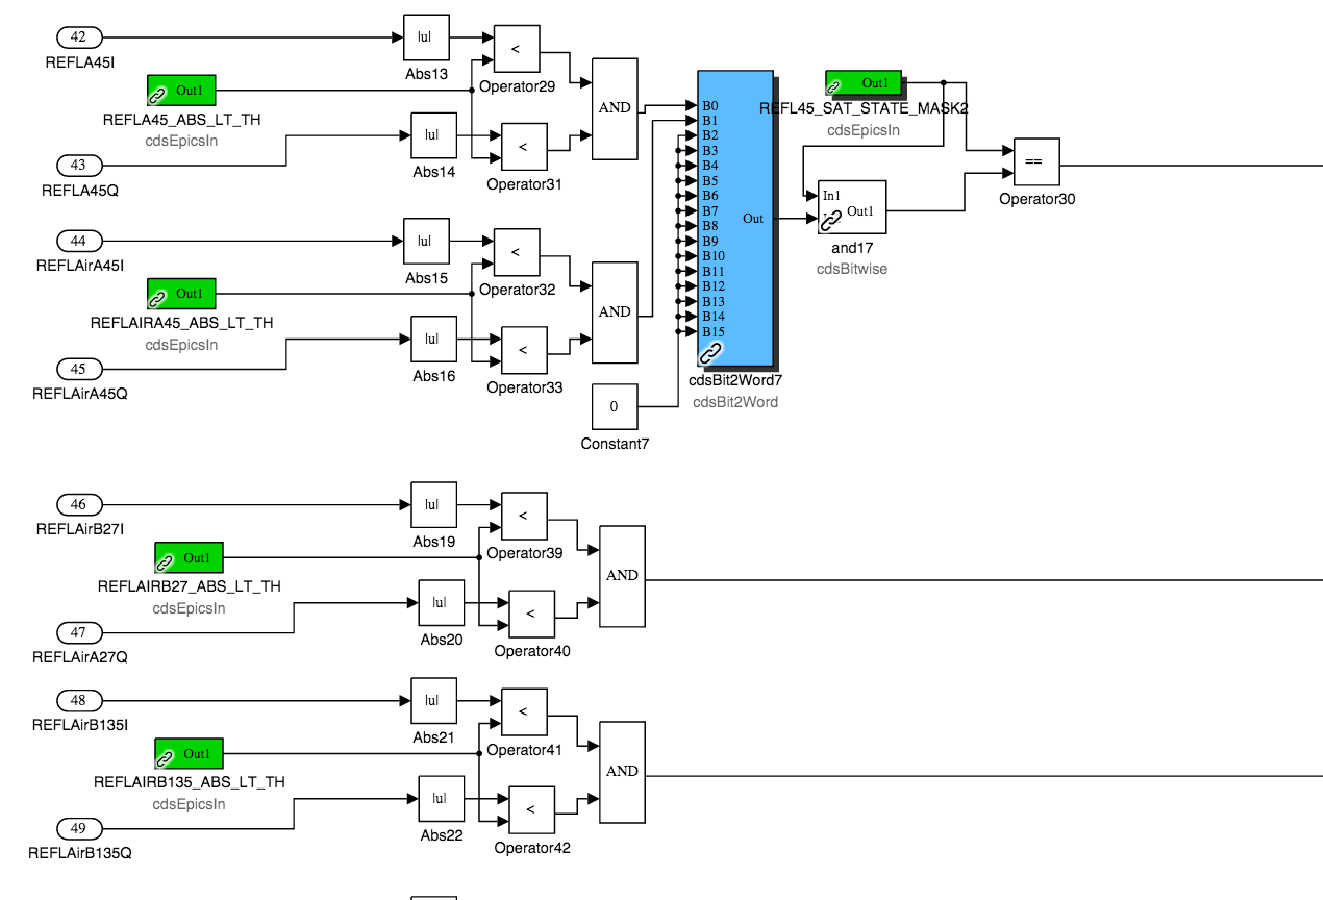
\includegraphics[width=\textwidth]{figures/ODC/LSC-ODC-model}
\caption[LSC ODC SIMULINK Model Example]{LSC ODC checks implemented in SIMULINK. %
         The numbered ovals on the left indicate signals used in real-time control %
         of the interferometer. The green boxes represent user-defined threshold %
         values to be used in boolean comparisons. The white boxes represent operations %
         such as computing the absolute value of a signal or performing boolean %
         comparisons (less than, greater than, AND, OR, etc.)}
\end{figure}\label{fig:lsc-odc-model}

Once the ODC model has performed all of its checks and reported a True or False 
answer, the information is stored in an overall state vector that can be parsed to 
learn the state of the LSC subsystem at any time. 
Figure \ref{fig:lsc-odc-bits} shows a visual representation of the state of the 
length degrees of freedom in the H1 interferometer over the course of a day.
Each horizontal bar represents the state of a length degree of freedom as 
reported by ODC. In this particular day, the control signals for the Michelson 
(MICH) and signal recycling cavity (SRCL) degrees of freedom exceeded their 
nominal range while the interferometer was in its nominal operating state. 
This is indicated by the color of the bars switching between 6:00 - 8:00 UTC 
and between 14:00 - 16:00 UTC. All of the times when the state changes are 
recorded as time segments which can be used to correlate excursions in the 
cavity control signals with transients in the output of the interferometer. 

\begin{figure}[ht!]
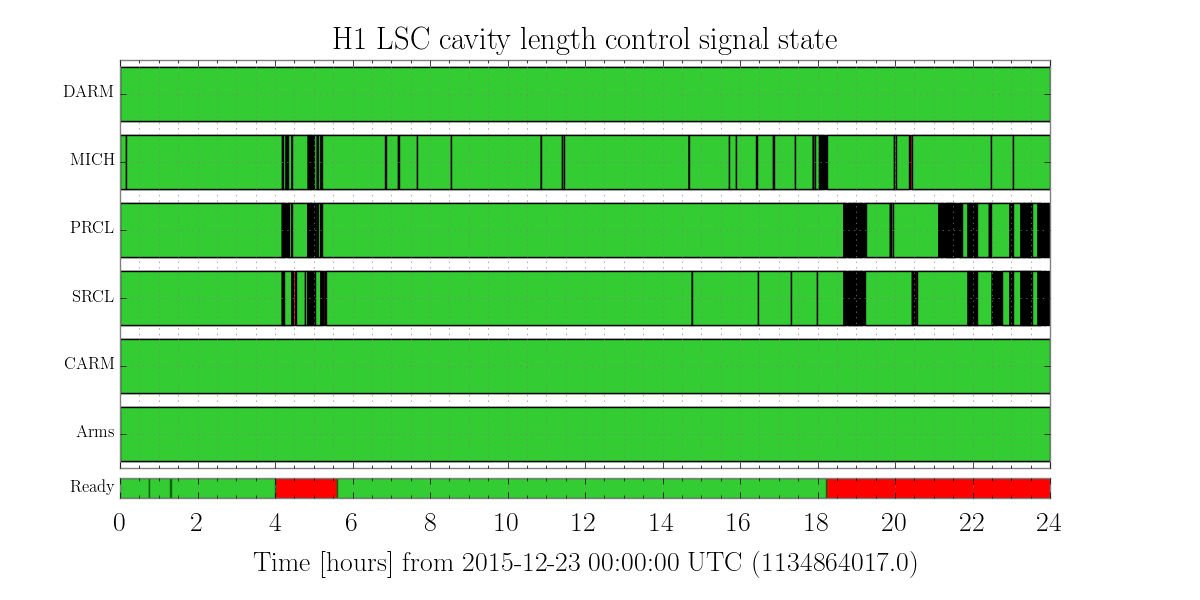
\includegraphics[width=\textwidth]{figures/ODC/LSC-bit-example}
\caption[LSC ODC bits example]{ODC bits representing states of length degrees of %
         freedom. Each horizontal bar represents a length degree of freedom that %
         is controlled in the LSC subsystem. When the bar is green, the control %
         signal for that degree of freedom is in its nominal range. When the %
         bar is not green, the control signal for that particular length degree %
         of freedom has exceeded the threshold set in the ODC model and is reported %
         as out of range.}
\label{fig:lsc-odc-bits}
\end{figure}

\subsection{MEDM screens}

For real-time use of these monitors, a software package called MEDM is used to 
display and interact with the ODC models. MEDM can be used to update the thresholds 
and state masks used to determine the status of a given photodiode or degree of 
freedom. 
Figure \ref{fig:lsc-odc} shows the LSC ODC overview screen in MEDM. 
The top panel summarizes the overall state of the subsystem, showing the state of 
each ODC bit and a bitmask that indicates whether or not a given bit is used in 
determining the overall state of the subsystem. 
The leftmost 
panel is used to monitor the state of each length degree of freedom in the interferometer. 
The rest of the panels are used to monitor the states of the various photodiodes used 
for sensing length degrees of freedom. These include DC power monitors and the values 
of RF demodulated photodiode signals. The grey boxes containing numerical values indicate 
user-set thresholds that can be updated from this screen.

\begin{figure}[ht!]
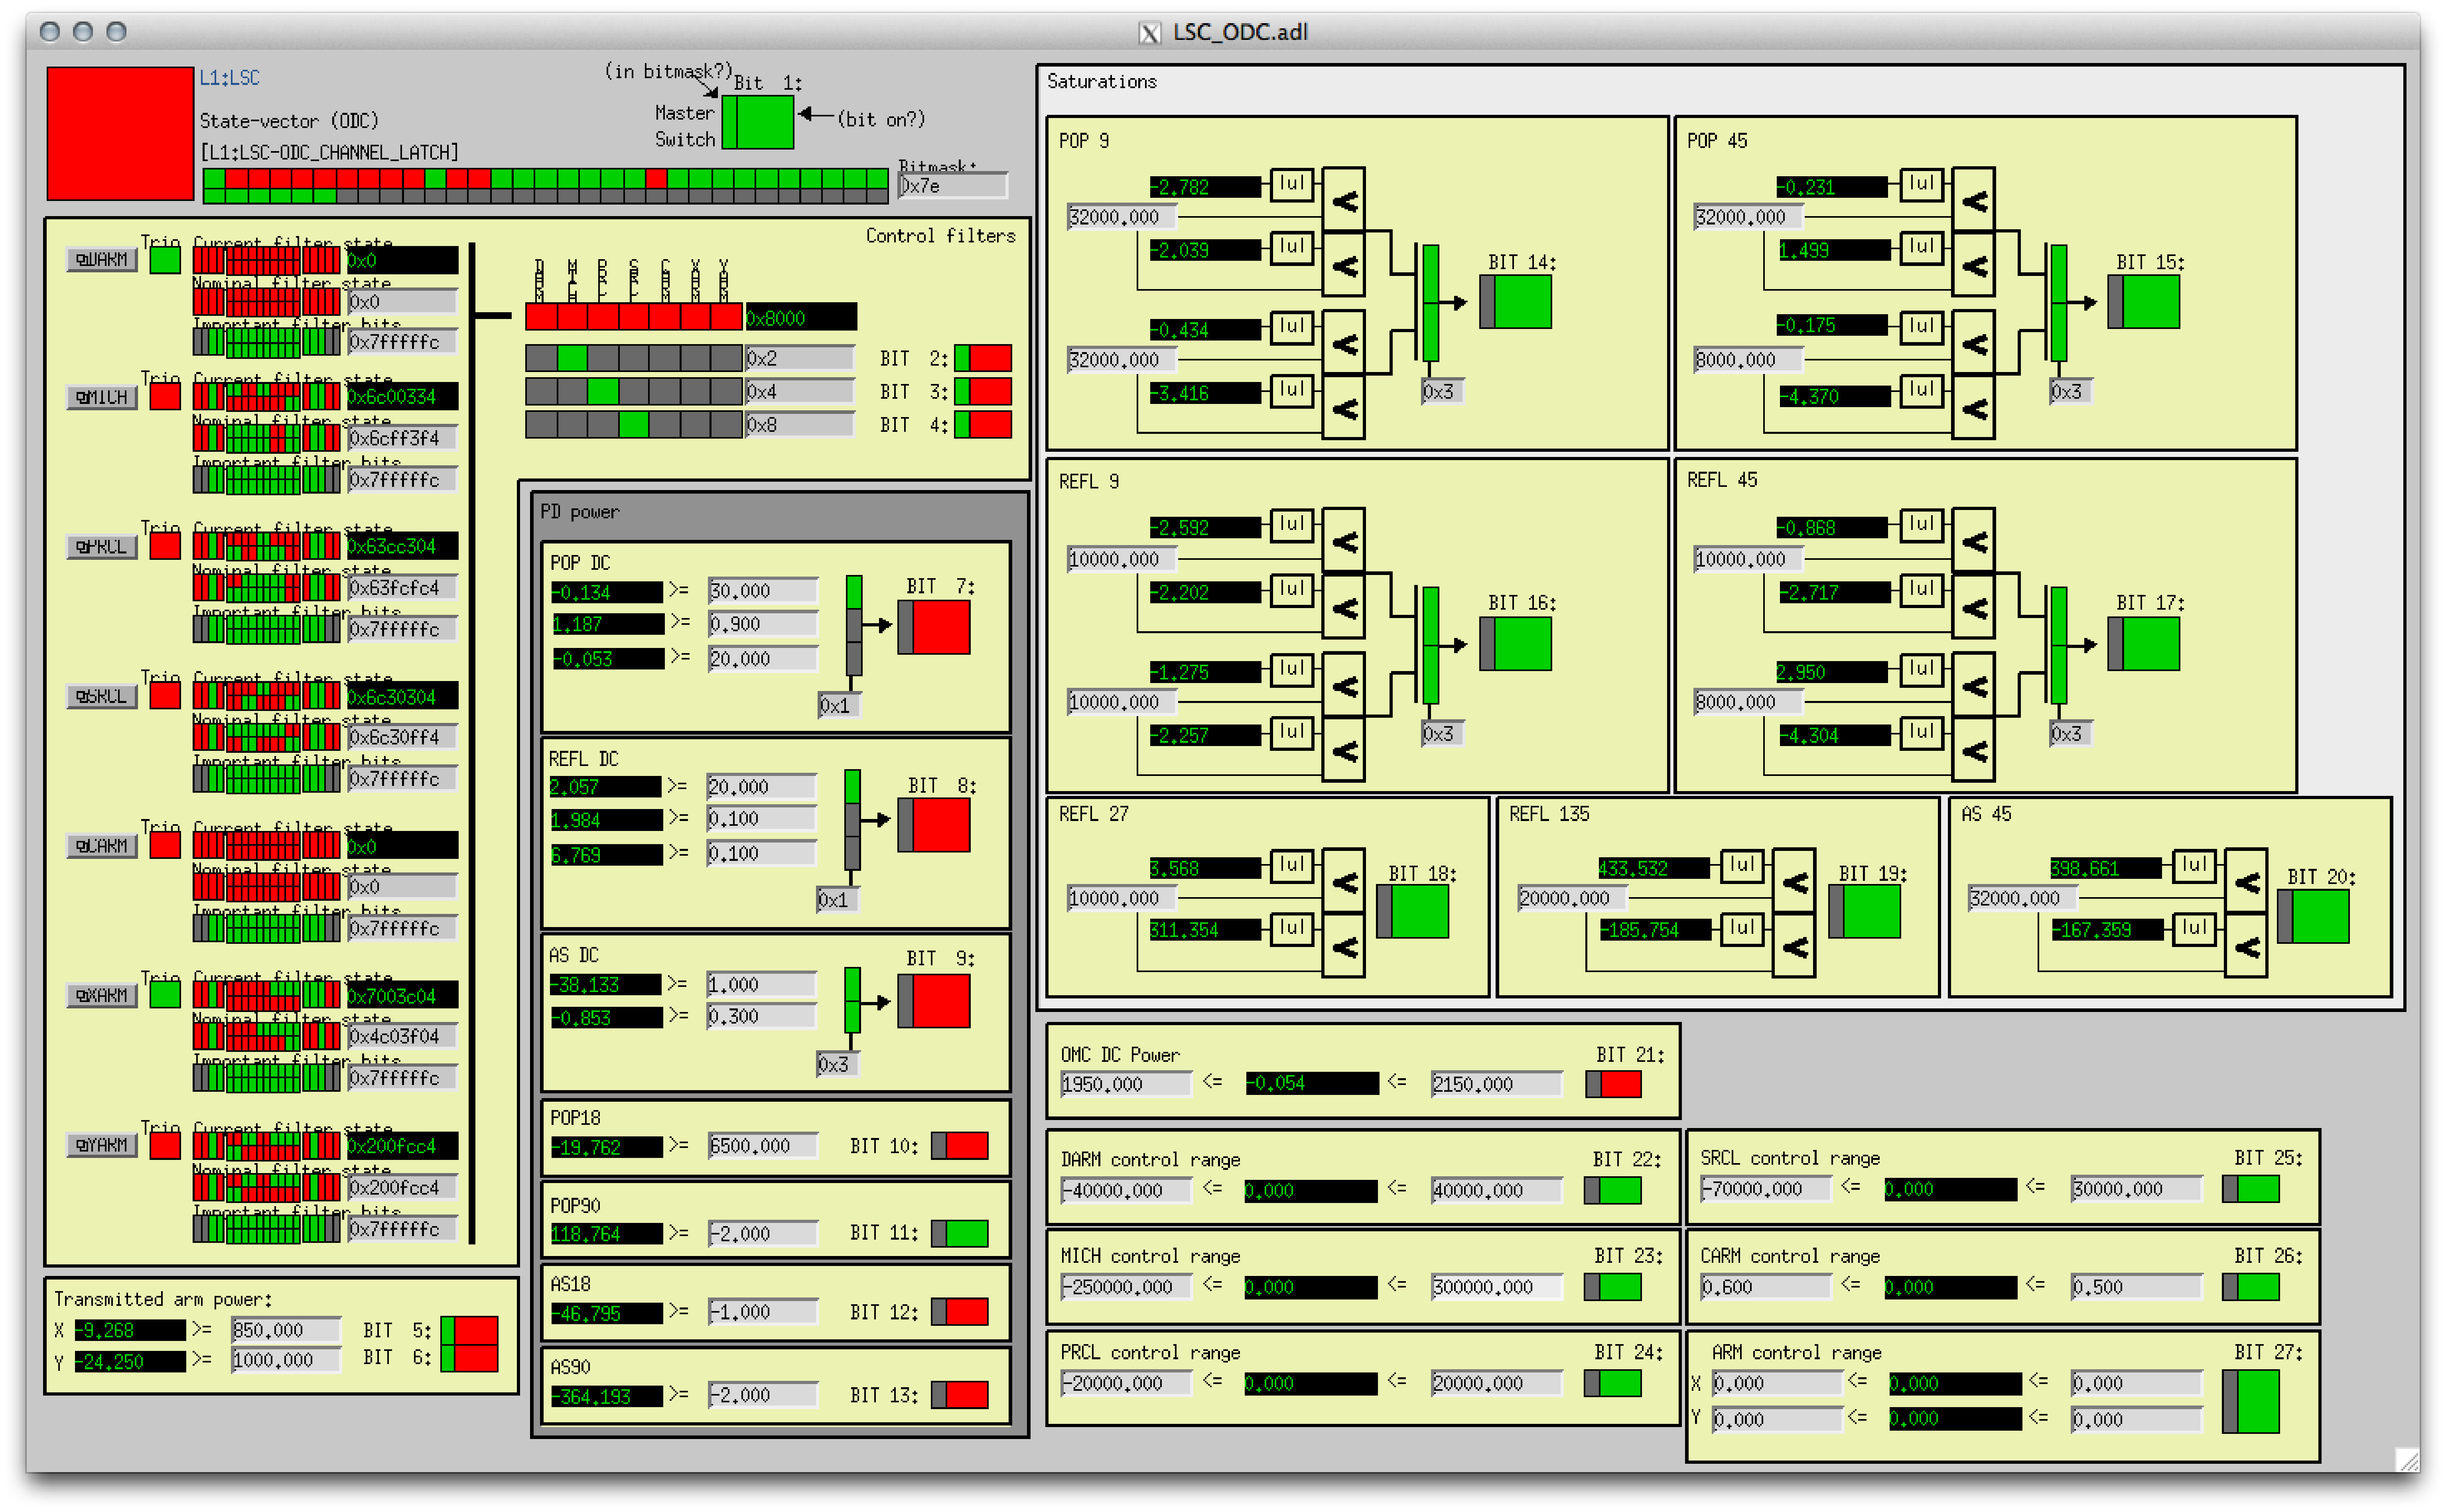
\includegraphics[width=\textwidth]{figures/ODC/LSC_screen}
\caption[LSC ODC Overview Screen]{MEDM screen used to interact with the LSC ODC model. %
         This screen contains information regarding the overall state of the LSC subsystem, %
         the state of control loops pertaining to specific length degrees of freedom in the %
         interferometer, and the state of photodiodes used to sense length degrees of freedom %
         in the interferometer.}
\label{fig:lsc-odc}
\end{figure}

\subsection{Summary pages}

While the MEDM screens are useful for real-time readout of the ODC models, they do not 
have an easily accessible history. For this reason, summary pages were built that 
contain the most important information from each ODC model. The summary pages are 
built multiple times per day and are accessible through a web browser, which allows 
easy, organized access to past interferometer data when performing a data 
quality investigation. 

Figure \ref{fig:lsc-odc-bits}, which shows the status of the length degrees of freedom 
of the interferomter over the course of a day, was taken from the summary pages. In this 
figure, the MICH degree of freedom was seen to move into a bad state during a locked state. 
As an example, we can look at the summary page visualization of the MICH degree of freedom 
during this time. 
Figure \ref{fig:mich-summary-pages} shows the control signal for the MICH degree of freedom 
with the ODC threshold 
overlaid as a dashed red line. The solid blue line indicates the median value of this signal 
over the course of 1 minute and the shaded regions indiate the maximum and minimum over 
this same stretch of time. When the control signal exceeds the ODC threshold, such as at 
about 14:35 UTC, the corresponding bit in Figure \ref{fig:lsc-odc-bits} flashes red to 
indicate the excess noise in this channel. 

\begin{figure}[ht!]
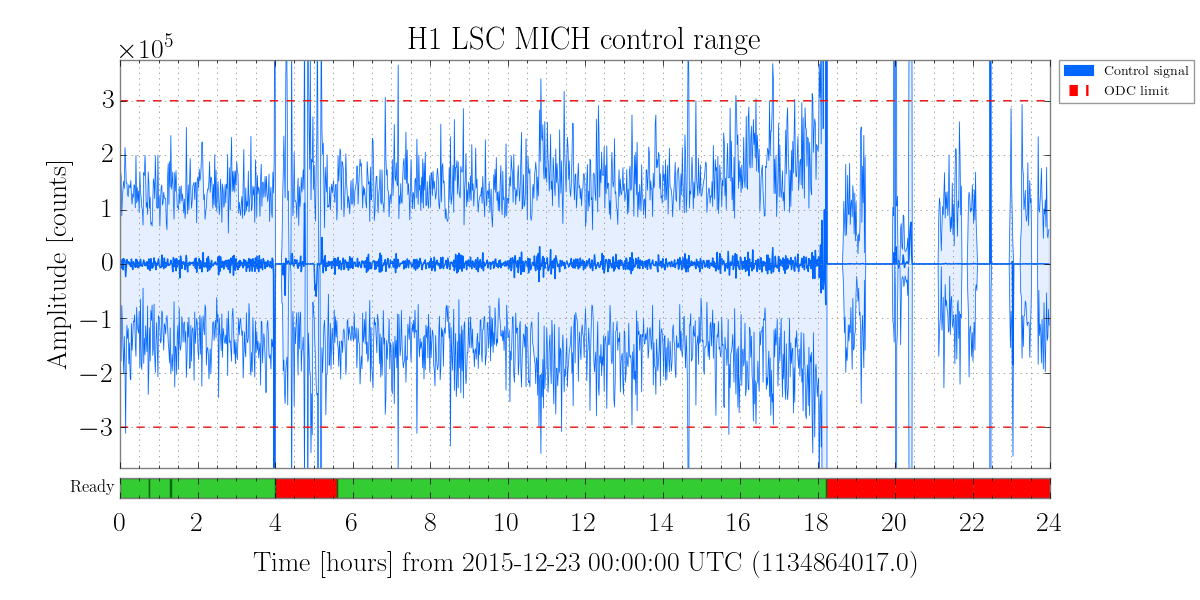
\includegraphics[width=\textwidth]{figures/ODC/H1-MICH-SUMMARY-PAGES}
\caption[MICH control signal on summary pages]{Readout of the MICH degree of freedom as %
         displayed on the summary pages. The dark blue curve indicates the median value of %
         the MICH control signal over the course of 1 minute. The shaded regions indicate %
         the maximum and minimum values of the control signal over the same stretch of time. %
         The dashed red line indicates the ODC threshold set to monitor this control signal.}
\label{fig:mich-summary-pages}
\end{figure}

\section{Alignment Sensing and Control}

The alignment sensing and control subsystem is used to control the alignment of 
optical cavities as well as the input pointing of light into those cavities. 
The control loops work in a similar way as the length sensing and control subsystem, 
using the reflected light from optical cavities to control the optics in a PDH 
scheme. The same set of RF sidebands that are used for length control are also used 
for alignment control. The detail that allows length fluctuations to be decoupled from 
alignment fluctuations is that alignment fluctuations generate higher order 
modes in the optical field, which are used in the demodulation stage to 
generate an error signal.

A length control loop compares the TEM00 mode of the carrier beam to the TEM00 
mode of the RF sidebands. 
An alignment control loop will compare the TEM00 mode of the carrier 
beam with the TEM10 and TEM01 modes of its sidebands, which are generated by 
angular misalignments of optical cavities. 
Since each optic has two alignment degrees of freedom that are directly 
controlled, pitch and yaw, and each cavity is comprised of multiple optics, 
the reflected light from each cavity is read out on a 
pair of quadrant photodiodes. This is visualized in Figure \ref{fig:odc-pd-screen}. 
The four quadrants allow the pitch and yaw error 
signals to be decoupled. Since higher order optical modes have a different Gouy 
phase as they propagate through space, a pair of photodiodes separated by a Gouy 
phase telescope are used to determine the origin of the misalignment 
(cite Nergis' thesis).

\subsection{Online Detector Characterization}

Given that the alignment sensing control subsystem is designed similarly 
to the length sensing and control subsystem, the general layout of the ODC 
model is very similar. The photodiodes signals used to generate alignment 
error signals are checked against a saturation threshold. The control 
signals that are sent to the optics are checked to ensure that they aren't 
exceeding their nominal range. Each degree of freedom is represented as one 
bit in a state vector, which can be compared to a series of state masks to 
check for a series of valid states. 

\subsection{MEDM screens}

The MEDM screens for the ASC subsystem are similar to those built to monitor 
the LSC subsystem. 
Figure \ref{fig:asc-odc} shows the ASC ODC overview screen in MEDM. 
The top panel once again describes the overall state of the subsystem and 
shows which ODC bits are used to determine that state. The left panel shows 
the status of the control signals used for each of the alignment degrees of 
freedom in both pitch and yaw. The bottom right panel, labeled 'QPD Saturations', 
checks for saturations in each of the quadrant photodiodes used in the ASC subsystem. 
Since there are many more checks that need to be made for the quadrant photodiodes, 
each one has a dedicated subscreen.

\begin{figure}[ht!]
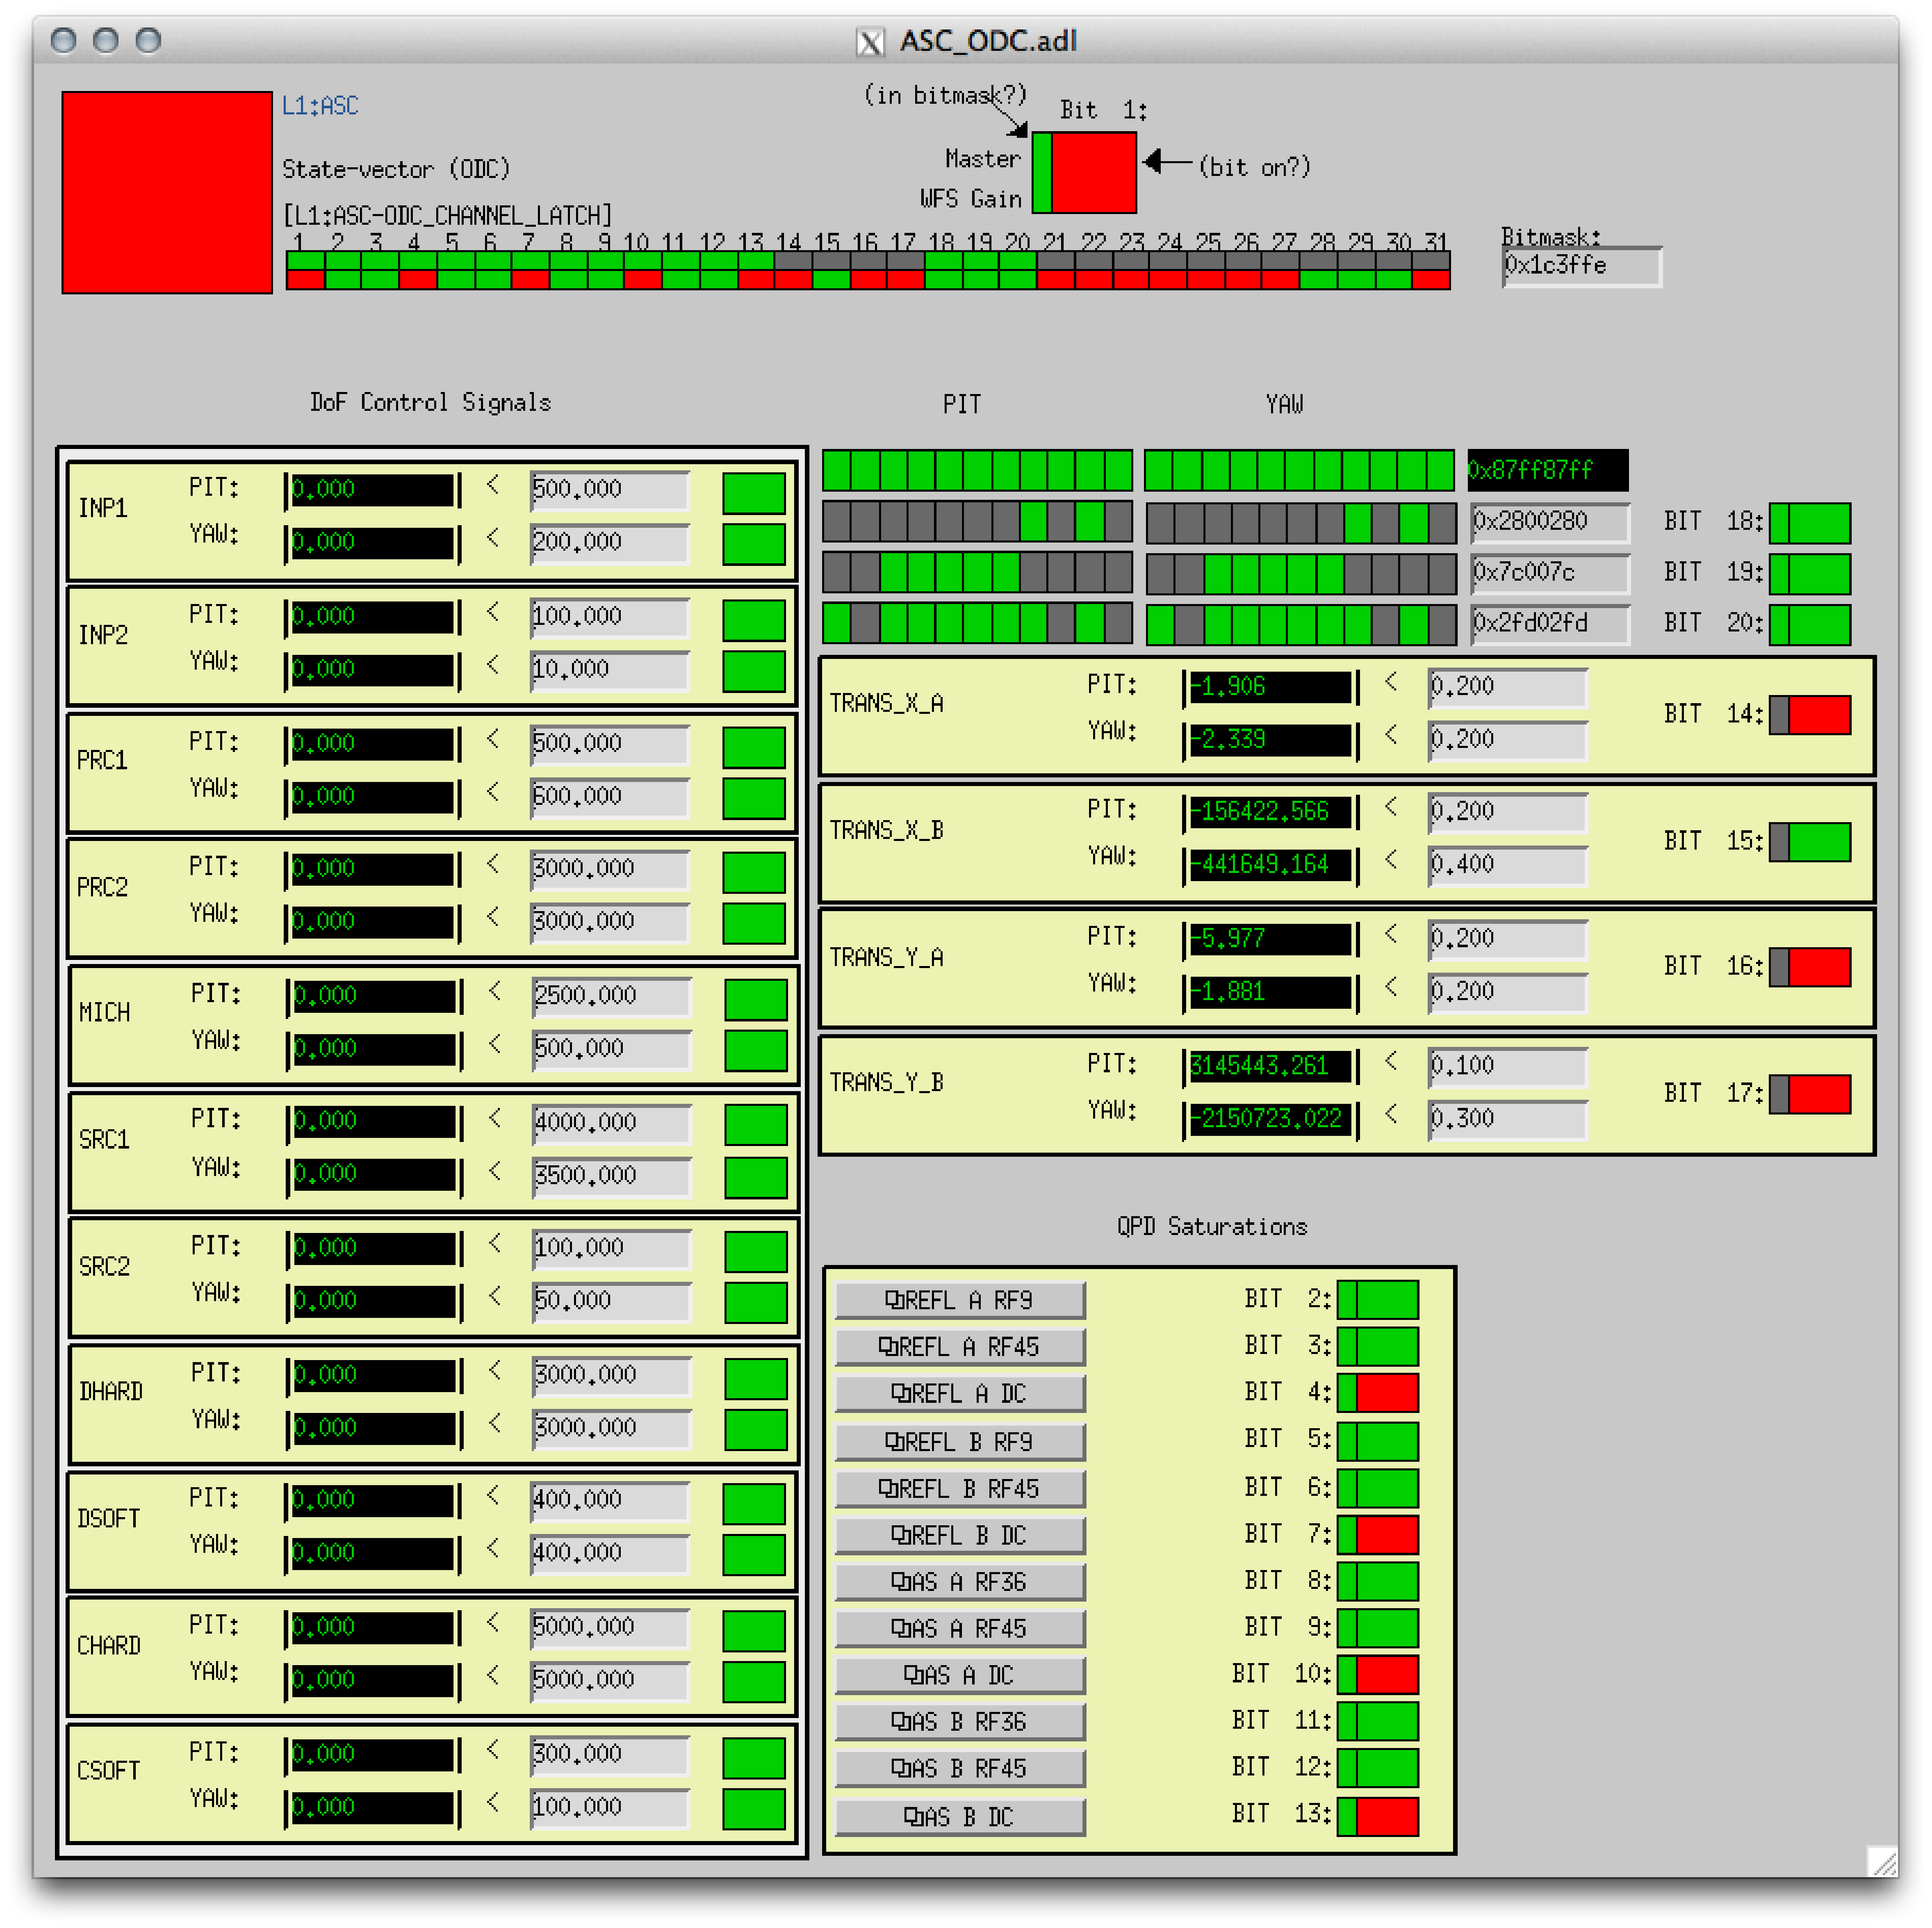
\includegraphics[width=\textwidth]{figures/ODC/ASC_screen}
\caption[ASC ODC Overview Screen]{MEDM screen used to interact with the ASC ODC model. %
         This screen shows the overall state of the ASC subsystem, the state of each %
         alignment degree of freedom in the interferometer, and the state of each %
         quadrant photodiode used to sense misalignments in the interferometer.}
\label{fig:asc-odc}
\end{figure}

Since the ASC subsystem uses quadrant photodiodes, each quadrant must be checked 
for saturation. 
Figure \ref{fig:odc-pd-screen} shows a photodiode monitor screen in the ASC ODC. 
The first and second panels show the readouts of each quadrant of a quadrant 
photodiode in I and Q phase respectively. The absolute value of each signal is 
calculated and compared to a threshold value to see if any quadrants are approaching 
a saturation limit. The third and fourth panels perform checks on the associated 
pitch and yaw readouts from these photodiodes to check for excursions beyond the 
nominal threshold. The nominal values for the pitch and yaw degrees of freedom 
are determined by trending these values over long durations of good interferometer 
performance.

\begin{figure}[ht!]
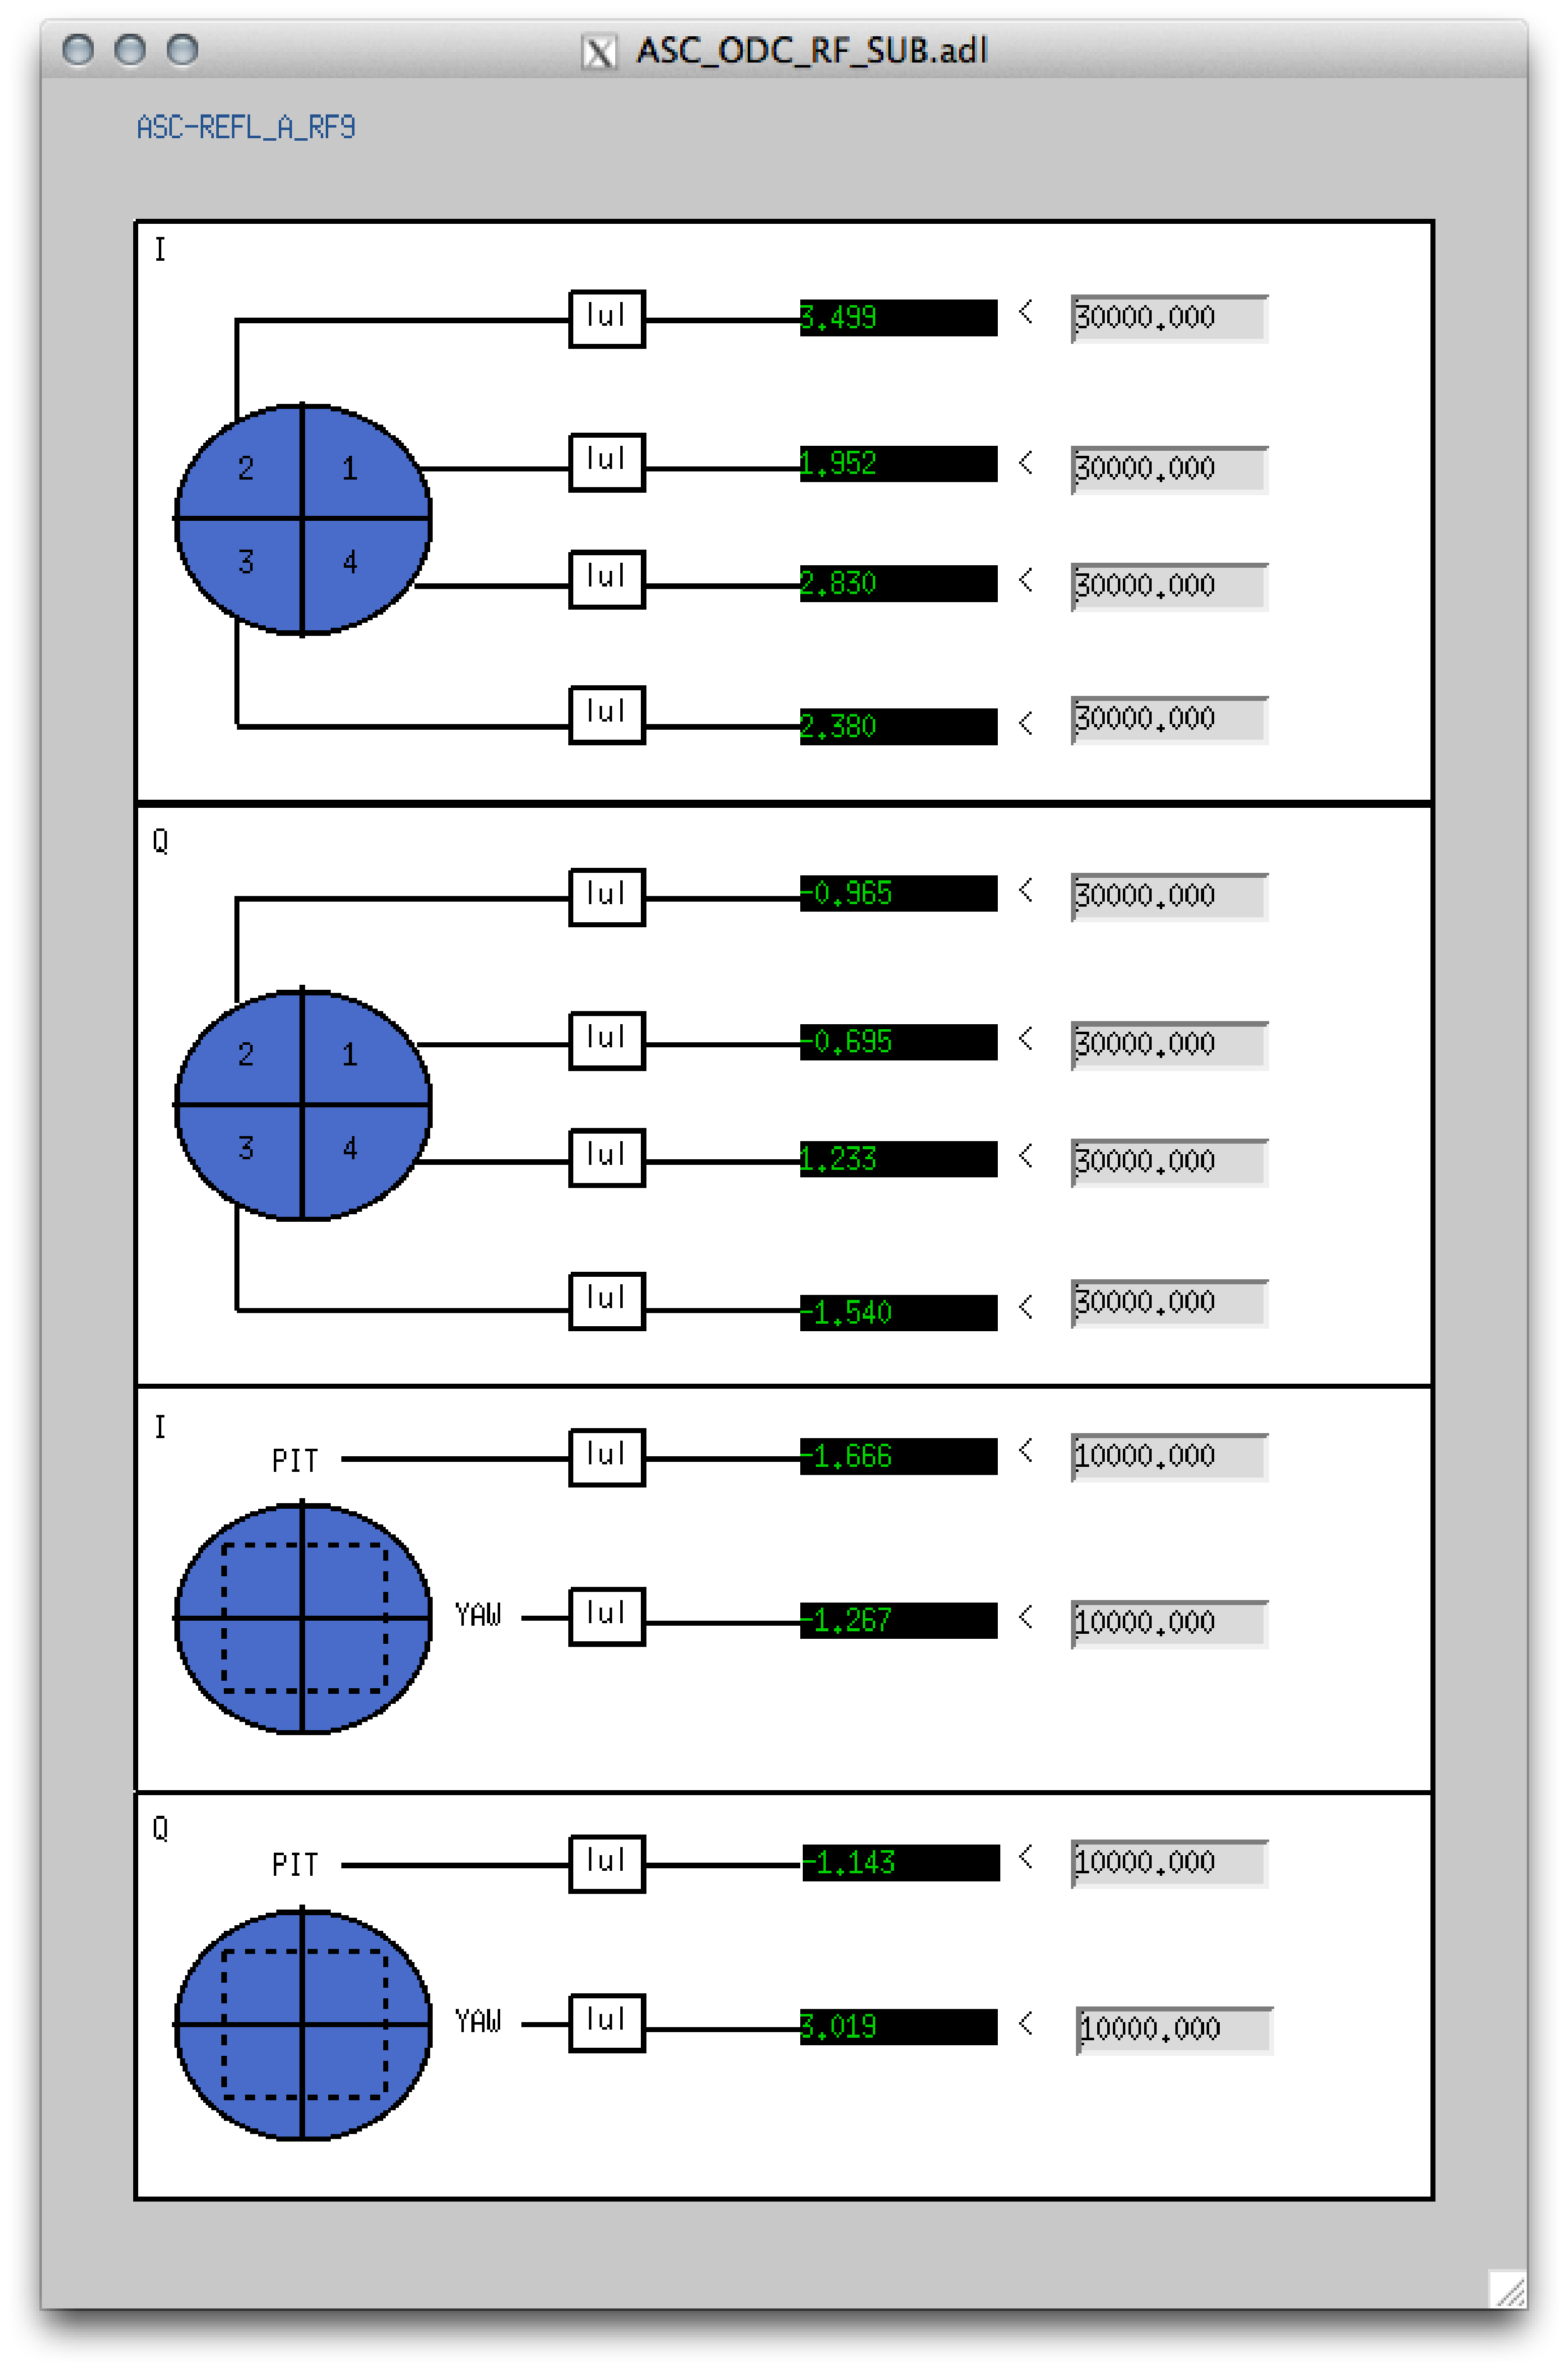
\includegraphics[width=0.7\textwidth]{figures/ODC/PD_screen}
\caption[ASC ODC Photodiode Monitor in MEDM]{ODC monitor for ASC photodiode in MEDM}
\label{fig:odc-pd-screen}
\end{figure}

\subsection{Summary pages}

The ASC subsystem also has an accompanying set of summary pages that keep a running 
record of its state. These summary pages are designed similarly to the LSC summary 
pages, including time-series of the control signals for each alignment degree of freedom, 
saturation monitors for the ASC photodiodes,  
and ODC plots indicating the state of each degree of freedom.

\section{ODC Results}

The ODC system was designed and implemented in the engineering runs that preceded the 
first observing run. During the first observing run, the first efforts were made to 
use the information reported by the ODC models to flag and understand noisy data. 
The most useful 
used the excess noise in the Michelson pitch degree of freedom to flag upstream 
electronics issues that caused loud glitches in $h(t)$. There is also evidence 
that the overall alignment status reported by the ASC ODC can be used as an early 
warning that the interferometer is going to drop out of its nominal operational 
state.

\subsection{MICH ODC as a witness of RF45 glitches}

The ODC channel built to monitor the Michelson (MICH) pitch degree of freedom 
was used to generate vetoes used in O1 analyses. Throughout O1, the H1 
interferometer was prone to a glitch mechanism driven by malfunctions in 
RF electronics used to generate frequency sidebands on the carrer beam. 
These RF sidebands are used to control auxiliary degrees of freedom in the 
interferometer, including the length of the small Michelson interferometer 
formed by the beamsplitter and the two ITMs. When the RF electronics glitched, 
the error signals of these cavities would also glitch, causing excess motion 
in the auxiliary degrees of freedom that was witnessed by ODC monitors set 
up to monitor the control signal of the MICH alignment control loops. 

Figure \ref{fig:mich-odc-example} 
shows the correlation between the witness channel for this ODC channel 
and glitches in $h(t)$ as identified by Omicron. Figure \ref{subfig:mich-odc-timeseries} 
shows a timeseries the control signal of the MICH pitch control loop. The ODC threshold, 
set at a value of 250 for this particular channel, is indicated by the green dotted 
line. Any time the control signal crosses this threshold, a segment is created to 
indicate that the control loop is not in a nominal operating state. Figure 
\ref{subfig:mich-odc-omicron} shows the $h(t)$ Omicron triggers over the same 
duration. When the MICH pitch control point has a high variance, for example 
in the first 1.5 hours of the plot, there is an 
overall increase in the rate of high SNR Omicron triggers, indicating that 
this ODC channel is witnessing alignment fluctuations that couple into the 
output of the interferometer. 

\begin{figure}[ht!]%
\subfloat[]{
  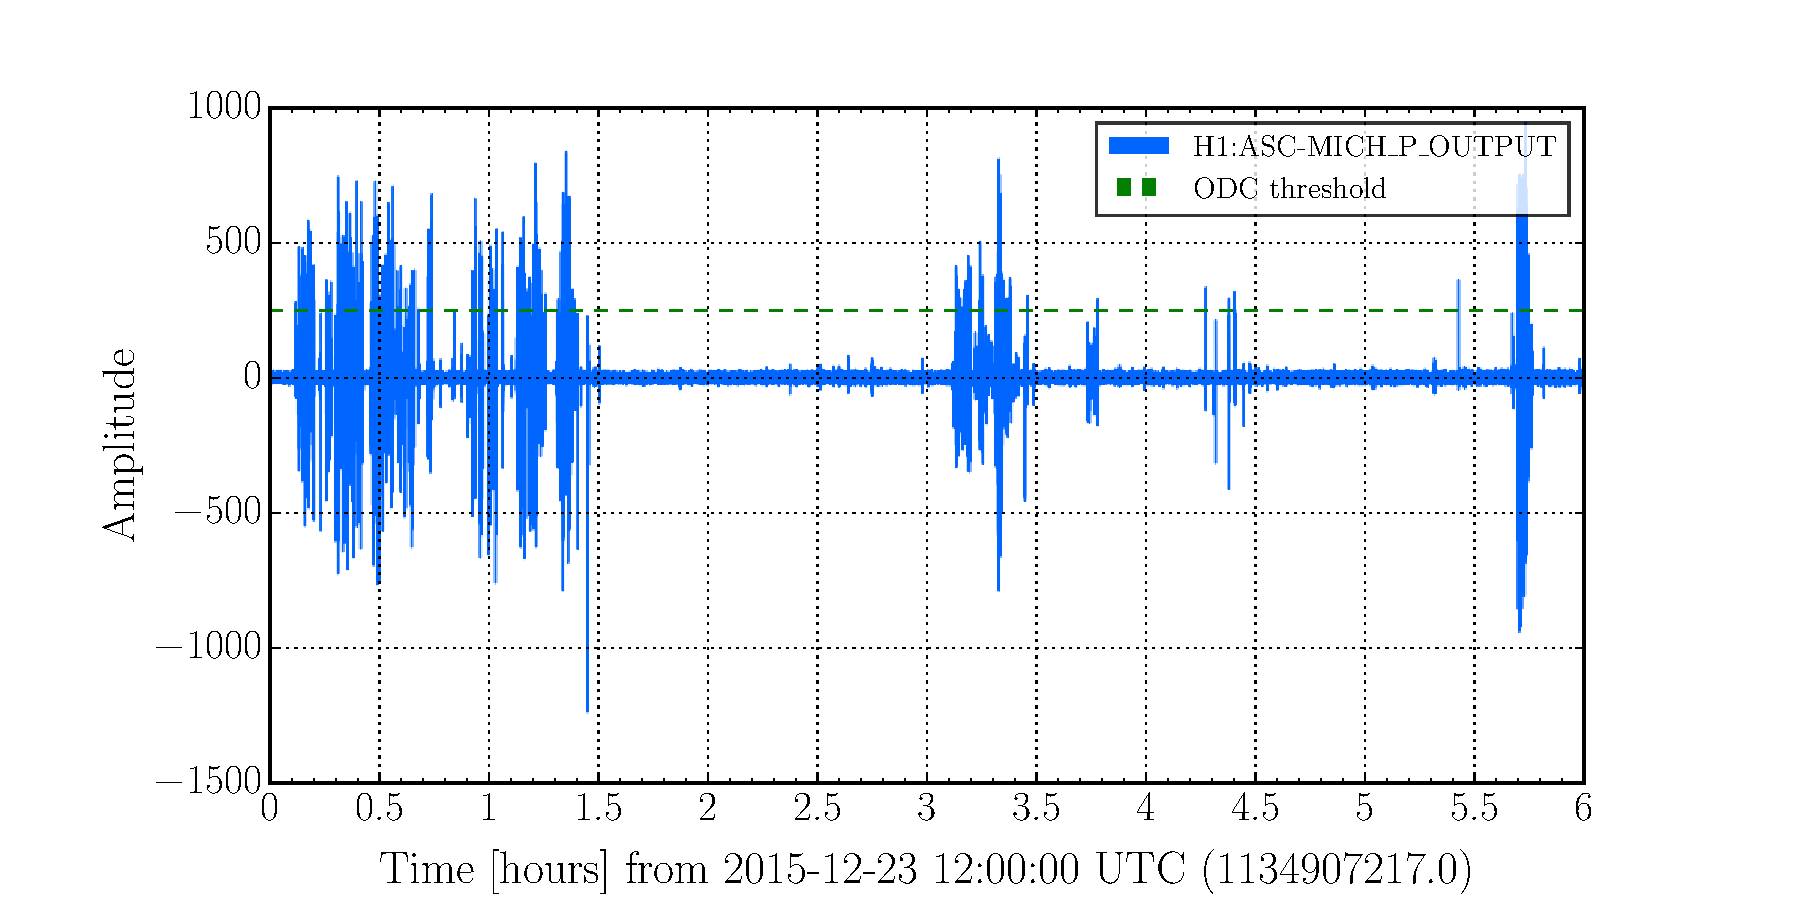
\includegraphics[width=\textwidth]{figures/detchar/MICH_P_OUTPUT_ODC}
  \label{subfig:mich-odc-timeseries}
  }

\subfloat[]{
  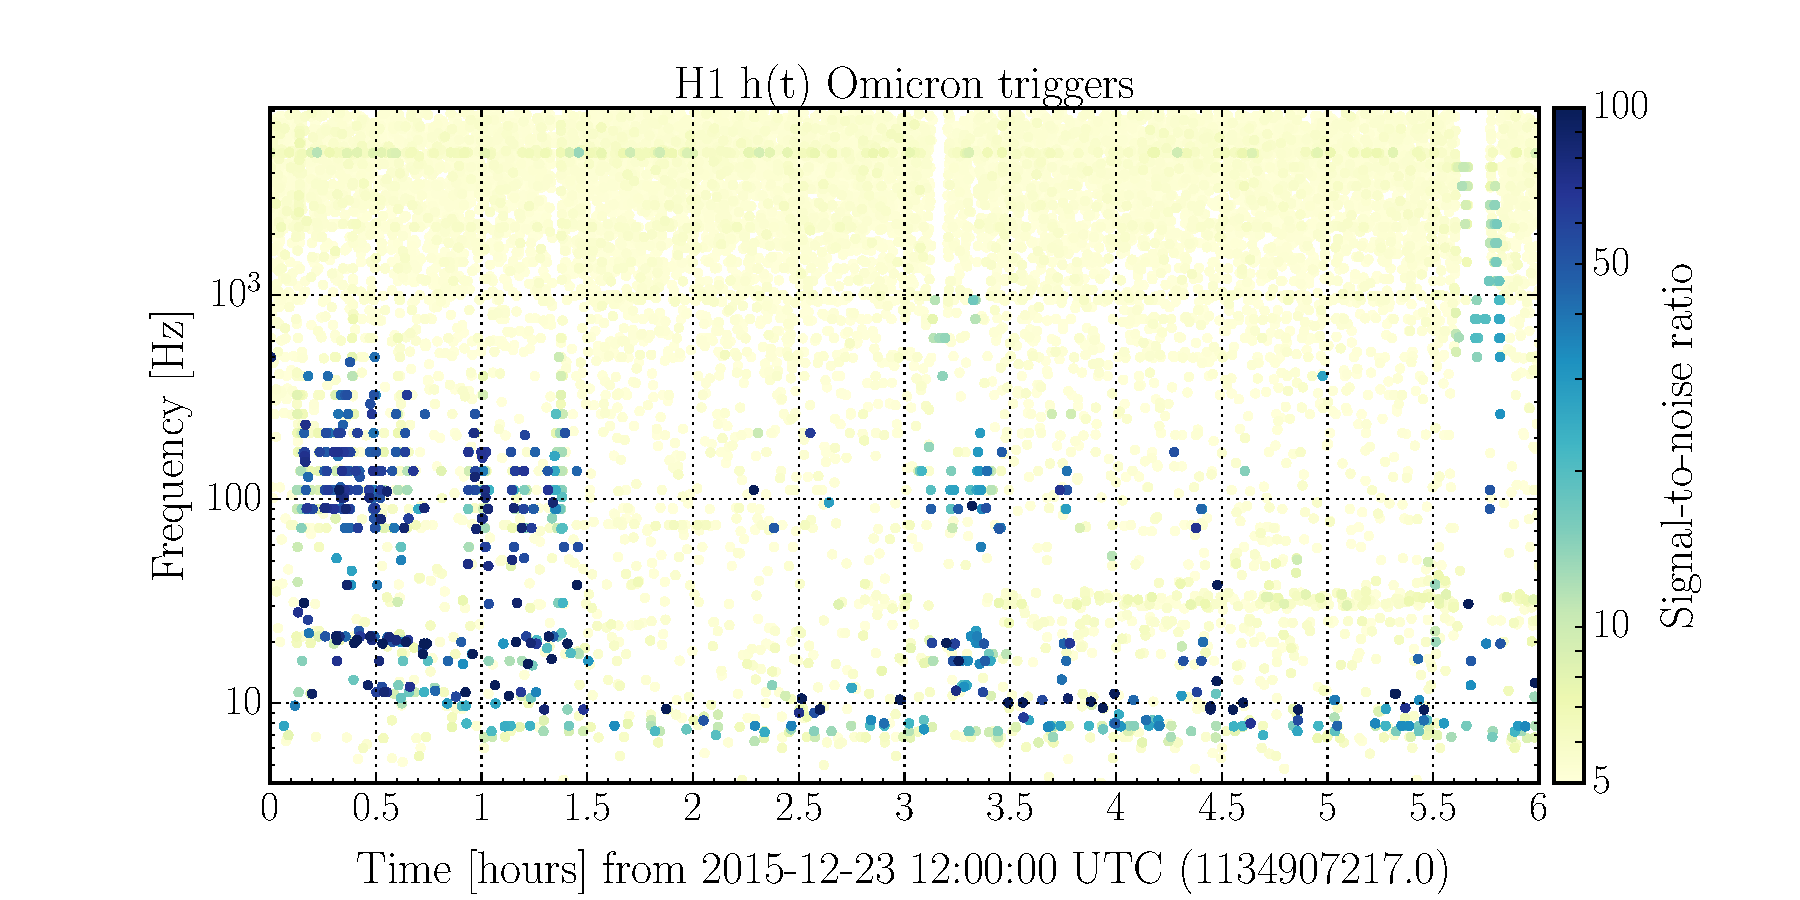
\includegraphics[width=\textwidth]{figures/detchar/Omicron_MICH_ODC}
  \label{subfig:mich-odc-omicron}
  }
\caption[ODC threshold on MICH pitch]{%
         An example of an ODC channel witnessing RF electronics issues, which %
         manifested as angular fluctuations in the vertex degrees of freedom %
         at H1. Figure \ref{subfig:mich-odc-timeseries} shows the ODC threshold %
         marking fluctuations in the MICH pitch degree of freedom. Figure %
         \ref{subfig:mich-odc-omicron} shows the associated Omicron triggers from %
         $h(t)$ at the same time. The storms of loud triggers between 10 - 400 Hz %
         are coincident with times flagged by this ODC monitor.}
\end{figure}\label{fig:mich-odc-example}

This coupling can be quantified using the veto evaluation tool (VET). The 
segments generated by this ODC channel are very efficient at vetoing high SNR 
Omicron triggers. VET reports that these segments veto Omicron triggers with SNR 
$>$ 8 with an efficiency:deadtime ratio of 47.16, indicating that these segments 
veto a large number of high SNR Omicron triggers with very little deadtime. These 
veto segments were included in the veto definer files that were distributed to 
the CBC and Burst searches in O1. 



%\Chapter{Conclusion}
%\label{ch:conclusion}
%\section{Summary}

aLIGO has begun taking data and will achieve design sensitivity over the next few years. At that point, the next generation of upgrades and improvements must be nearly ready to implement. One possible such upgrade would be to damp the unwanted angular motion in the test masses using radiation pressure feedback. This has the potential benefits of reducing the angular noise of the system and thus also reducing the amount of noise that couples from angular motion into cavity length.  
 
We have explored the implementation and uses of radiation pressure feedback, optical springs, to control the motion of a mirror. 
We demonstrated in several ways the underlying principles and behavior of optical springs, in both straight and folded cavities.
We discussed the mechanical design of the experiment, with the addition of blade springs to reduce the influence of seismic noise on the experiment.
We reviewed the feedback and controls in use for the optical traps. 
We measured and modeled the causes and effects of the photothermal effect in an optical spring system.
We explored one- and two-degree-of-freedom traps, and, while we could not get the angular trap stably locked for more than two seconds, we have laid out the path to do so.
We designed and modeled a full-scale implementation of angular optical springs to damp the Sidles-Sigg instability in the aLIGO configuration.

These developments should lay a strong groundwork for continued research into the applications and uses of radiation pressure feedback in aLIGO and beyond.

\section{Future work}

There are several things left unfinished that will hopefully deliver interesting results:

\begin{enumerate}
	\item Improving the stability  of the SU angular optical trap experiment and damping the 66 Hz resonance that seems to be preventing extended locks.
	There are a number of possibilities to increase the bandwidth and damp the motion outlined in Section \ref{sec:bandwidth}.
	\item Exploring the possibility of a a single stable optical spring with a specialized optical coating.
	We expect that dielectric coating manufacturers could do a custom run with a very thick first layer to create a ``self-locking'' cavity. The mirror could be mounted using the same cold weld method described in Section \ref{sec:endMirror}, then tested with the single-mirror input coupler from Chapter \ref{ch:photothermal}. 
	\item Designing and demonstrating a large scale angular trap in aLIGO.
	A detailed noise budget needs to be drafted using a modified version of GWINC or a similar tool to insure that we would not be introducing too much thermal noise.
	After that, a prototype of the design would need to be built at e.g. the Caltech 40 m interferometer to develop control systems and test predictions.
\end{enumerate}

%For each bullet, add at lease one more sentence that discusses how you would go about these items.
%What is the first thing to be done? What hardware needs to be purchased, changed? Etc.


%% $Id$
%
%Although the upper limit that we have placed on the rate of binary black hole
%MACHO inspirals in the galaxy is lower than the upper bound of the predicted
%rates, the LIGO interferometers were not at design sensitivity when the S2
%data was taken. At present, the sensitivities of the instruments are
%significantly better than during S2, as can be seen from
%figure~\ref{f:s3strain}, and progress on reducing noise in the interferometers
%continues apace.  The increase in detector sensitivity makes a larger volume
%of the Universe accessible to searches for binary inspirals. In addition to
%this, the amount of data is also increasing as the interferometers become more
%stable.
%
%These improvements in the instruments will increase the chance of detecting
%gravitational waves from binary inspirals. If the rates of binary black hole
%MACHO coalescence are truly as high as predicted, then initial LIGO would
%stand an excellent chance of detecting an inspiral. The first detection of
%gravitational waves will be a major scientific breakthrough and will yield and
%enormous amount of scientific information, particularly if the detection came
%from a binary black hole MACHO. The length of binary black hole MACHO
%inspirals in the sensitive band of the interferometer will allow extremely
%accurate parameter estimation as well as tests of post-Newtonian theory. For
%systems with total mass greater than $\sim 0.64\,\mathrm{M}_\odot$ LIGO will
%be sensitive to the coalescence of the binary and will be able to study the
%strong gravitational field effects when two binary black holes merge. When
%this is coupled with the accurate parameter estimation available from the
%earlier part of the waveform, the inspiral of a binary black hole MACHO could
%be an excellent laboratory for General Relativity.  A detection would also
%impact the studies of halo dark matter and early universe physics, providing a
%MACHO component to the halo and suggesting that primordial black holes do
%indeed form in the universe.
%
%In the absence of detection, the improvements in detector sensitivity will
%dramatically improve the upper limits placed on the rate of binary black hole
%MACHO inspirals. Once these rates are below the predicted rates, we may begin
%to use observations from gravitational wave interferometers to constrain the
%fraction of galactic halos in the form of primordial black hole MACHOs. While
%this may not be as significant as a detection, it will still be of interest to
%the astrophysical community.
%
%\newpage 
%
%\begin{figure}[p]
%\vspace{5pt}
%\begin{center}
%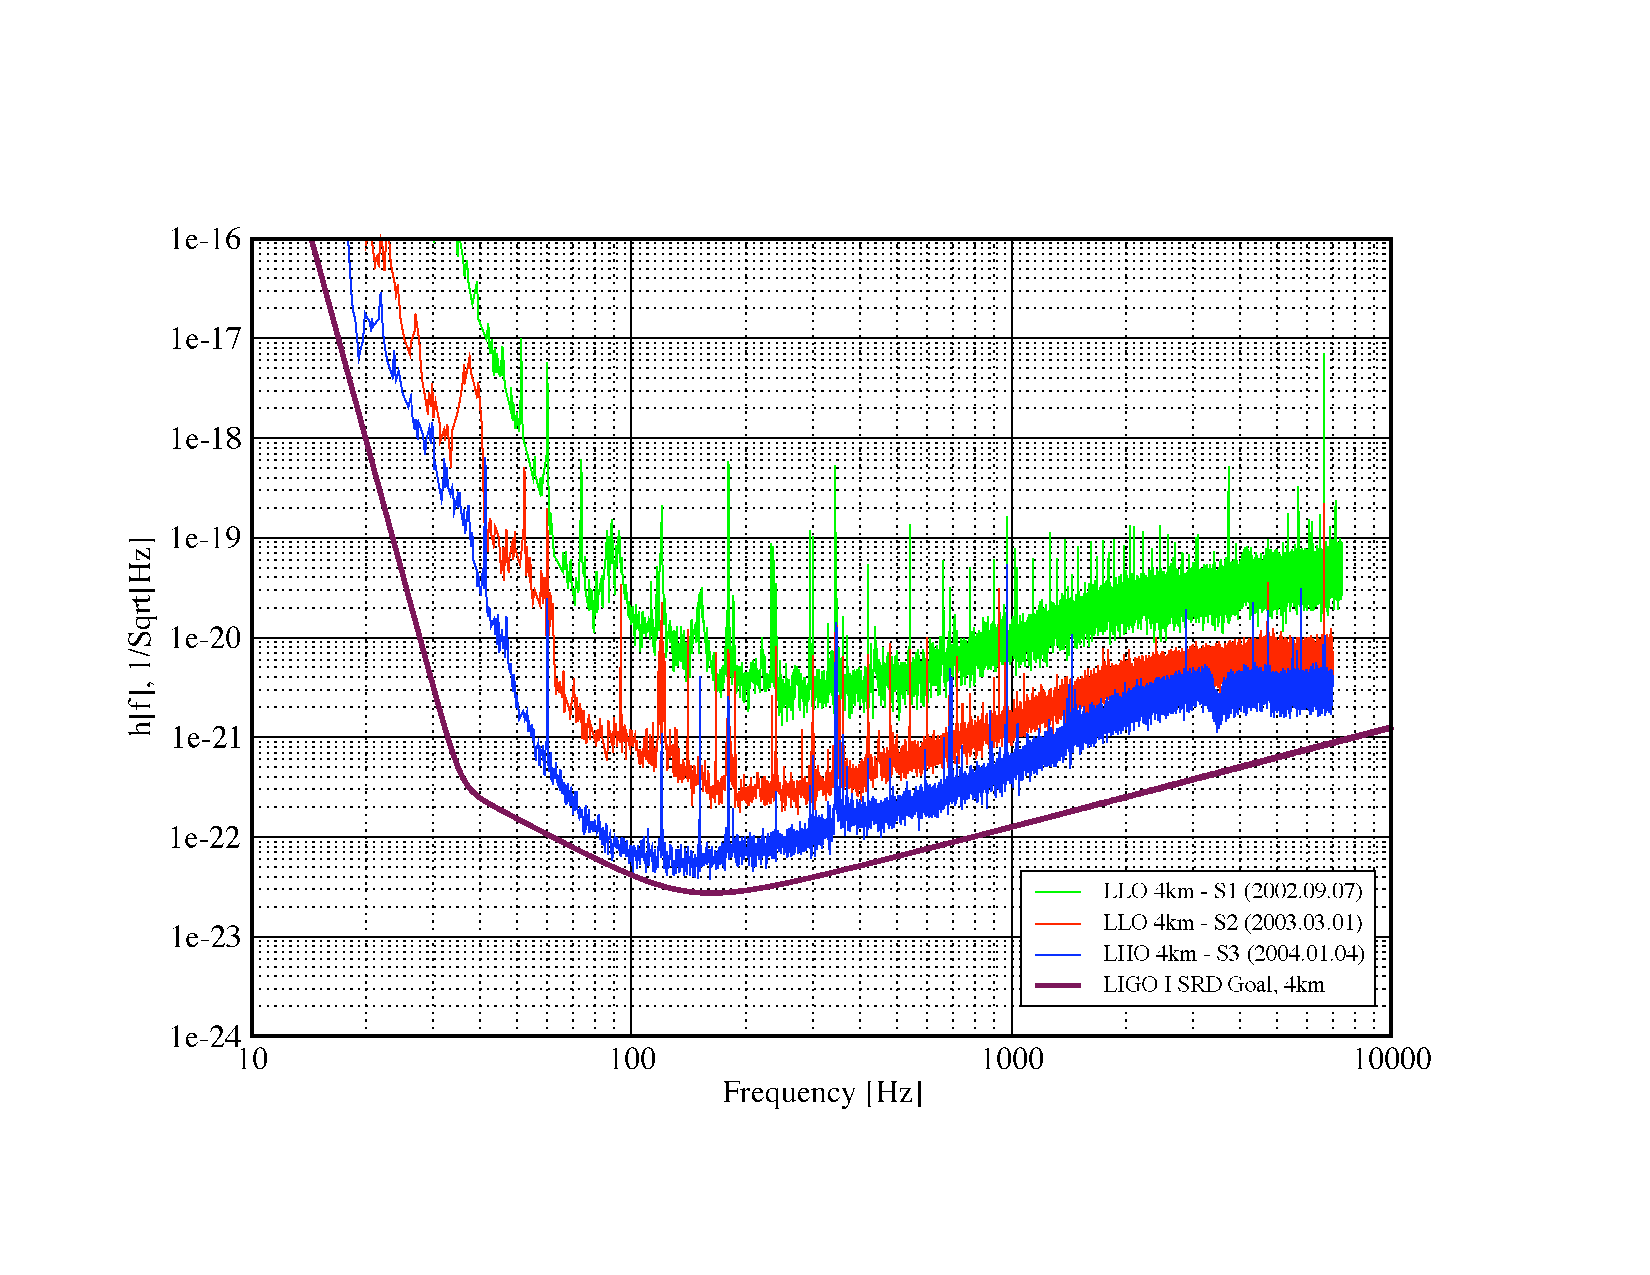
\includegraphics[width=\textwidth]{figures/conclusion/s3strain}
%\end{center}
%\caption[Comparison of Best LIGO Interferometer Sensitivity]{%
%\label{f:s3strain}
%Comparison of the best sensitivities of the LIGO interferometers between
%science runs. The solid curve shows the design sensitivity for the $4$~km
%interferometers: the LHO $4$~km is only a factor of $\sim 2$ away from design
%at $100$~Hz during S3.
%}
%\end{figure}
%


%\appendix
%\Chapter{Beam Separation}
%\label{ap:beamseparation}
%%\documentclass[12pt]{article}
%\usepackage{fullpage,graphicx}
%\title{Beam seperation}
%\author{David Kelley}
%\begin{document}
%\maketitle

\section{Definitions}
\begin{itemize}
\item $P_m$ Input power of the main beam 
\item $P_s$ Input power of the side beam
\item $f_m$ Main cavity finesse
\item $f_s$ Side cavity finesse
\item $R_c$ Radius of curvature of payload mirror (5 cm)
\item $\theta_m$ Main beam angle from optical axis.  Origin is at center of curvature.
\item $\theta_s$ Side beam angle from optical axis.  Origin is at center of curvature.
\item $c$ Speed of light
\item $R$ Payload mirror radius
\item $h$ Payload mirror thickness
\item $m$ Payload mirror mass
\item $I = \frac{m}{12}(3R^2+h^2)$ Payload mirror moment of inertia
\item $G = \frac{P_mf_m}{P_sf_s}$ Handy constant
\item $d = \theta_mR_c - \theta_sR_c$ Beam spot seperation
\end{itemize}


\newpage
\section{Balancing torques}
We want the mirror to be stationary, so the net torque on the mirror should be zero.

Force on payload mirror due to radiation pressure of the two beams:

$$ F_m = \frac{2P_mf_m}{c} \hspace{20 pt} F_s = \frac{2P_sf_s}{c}$$

$$\tau = F_m\theta_mR_c+F_s\theta_sR_c = 0$$

substituting in $d$,

$$\theta_m = \frac{d}{R_c(1+G)}$$

\section{Eliminating beam coupling}

We propose that there is a spot somewhere on the surface of the payload mirror where the sum of torque and force due to one beam makes the net force zero.  We place one beam spot at $r_1$.  We'd like to put the other beam in the null spot $r_2$ so that there is no force coupling between the two.  

$$Fs=\frac{2P_sf_s}{c} = m\omega^2x \hspace{20pt} x = \frac{F_s}{m\omega^2}$$ 
$$\tau_s = F_sr_1=I\omega^2\phi \hspace{20pt} \phi = \frac{F_s r_1}{I\omega^2}$$

Let's find a point these effects cancel:

$$r_2\phi-x=0 \hspace{20 pt} r_2=\frac{x}{\phi}=\frac{I}{mr_1}$$

It should be noted that the previously used $d$ can also be expressed as $d =r_2-r_1$.

$$r_2 = \theta_2R_c = \theta_mR_c$$

$$r_2 = \frac{d}{1+G}$$

$$\frac{I}{m} = \frac{(r_2-r_1)r_1}{1+G} = \frac{\left(\frac{I}{mr_1}+r_1\right)r_1}{1+G}$$

$$r_1 = \sqrt{\frac{I}{mG}} \hspace{20pt} r_2 = \sqrt{\frac{IG}{m}}$$

These radii are the ideal horizontal distances from the payload mirror optical axis to the beam spots.
%A MATLAB script that computes this seperation is included in this directory, named cavityAngles.m. 



%\end{document}

\clearpage
\bibliographystyle{unsrt}
\bibliography{references}

\addcontentsline{toc}{chapter}{\numberline {Bibliography}}

\clearpage
\birthplacedate{Rochester, NY \>\>July 22, 1989}
\collegewherewhen{%
\>Utica College \>\>2007--2011, \>B.S.\\
\>\su	\>\>2011--2016, \>Ph.D.}

\newpage
\null\vskip1in%
\begin{center}
{\Large\bf Curriculum Vitae}
\end{center}
\vskip 2em
\begin{tabbing}
\tabset
Title of Dissertation\\
\>Detector Characterization of Advanced LIGO
\end{tabbing}
\vskip 1em

\begin{startvita}
\end{startvita}

\renewenvironment{thebibliography}[1]%
  {\begin{list}{\labelenumi\hss}%
     {\usecounter{enumi}\setlength{\labelwidth}{3em}%
      \setlength{\leftmargin}{5em}}}%
  {\end{list}}
\renewcommand{\bibitem}[1]{\item\label{#1}\relax}%
\renewcommand{\theenumi}{\arabic{enumi}}%
\begin{publications}
\putbib[papers]
\end{publications}


\finishvita
\end{document}
